\documentclass[10pt,journal,compsoc]{IEEEtran}
%compsoc, transmag, comsoc; conference,journal
% *** CITATION PACKAGES ***
%
\ifCLASSOPTIONcompsoc
  % The IEEE Computer Society needs nocompress option
  % requires cite.sty v4.0 or later (November 2003)
  \usepackage[nocompress]{cite}
\else
  % normal IEEE
  \usepackage{cite}
\fi
\usepackage{amsmath}
\usepackage{amssymb}
\usepackage{amsthm}
\usepackage{graphicx} 
\usepackage{booktabs}
\usepackage{url}
\usepackage{xspace}
\usepackage[norelsize, linesnumbered, ruled, lined, boxed, commentsnumbered]{algorithm2e}

\usepackage[pagebackref=true,breaklinks=true,bookmarks=false,citecolor=blue,linkcolor=blue]{hyperref}
\usepackage{pifont}
\newcommand{\figoverview}{
\begin{figure}[tbp]
\begin{center}
\includegraphics[width=0.9\linewidth]{images/overview_zhou}
\end{center}
\caption{\textbf{GAN 逆向的图解.} 不同于传统的使用预训练的生成器$G$的采样和生成过程, GAN 逆向问题是把一个给定的真实图片$x$ 映射到隐空间中并且得到隐向量$\mathbf{z^{*}}$. 之后重建的图像$x^{*}$ 来自$x^*=G(\mathbf{z^{*}})$. 通过沿着不同方向改变隐向量 $\mathbf{z^{*}}$,我们可以编辑真实图像的相应属性. 比如,方向指定为$\mathbf{z^{*}}+\mathbf{n_1}$ 和$\mathbf{z^{*}}+\mathbf{n_2}$ ,其中$\mathbf{n_1}$ 和 $\mathbf{n_2}$ 分别在隐空间中模拟年龄和微笑. 重建结果来自\cite{zhu2020indomain}.
}
\label{fig:overview}
\end{figure}
}

\newcommand{\figtype}{
\begin{figure}[tbp]
\begin{center}
\includegraphics[width=0.95\linewidth]{images/inversion_types}
\end{center}
\caption{\textbf{GAN 逆向方法的图解.} 
(a) 给定一个训练良好的GAN模型,可以从随机采样的隐向量中生成逼真的图像. 
(b) {\bf 基于优化的} 逆向使用优化算法迭代优化隐向量,以最小化像素级重建损失. 
(c) {\bf 基于学习的} 逆向建立一个编码器网络,将图像映射到隐空间. 
(d) {\bf 混合} 方法使用编码器生成一个优化的初值,比如,首先利用编码器网络获取近似嵌入,然后用优化算法对其进行优化.}
\label{fig:inversion_types}
\end{figure}
}

\newcommand{\figwalk}{
\begin{figure}[t]
\centering
\includegraphics[width=1\columnwidth]{images/walk.pdf}
\caption{在隐空间中发现可解释方向的图解~\cite{jahanian2020steerability}. 
目标是找到一条 $\mathcal{Z}$ 空间中的路径来转换生成的图像 $G(\mathbf{z})$ 到它编辑过的版本 $\texttt{edit}(G(\mathbf{z},\alpha))$, 比如, an $\alpha \times$ 放大. 
这个变换可以由线性漫步$G(\mathbf{z}+\alpha \mathbf{w})$非线性漫步$G(f(f(...(\mathbf{z})))$表示.}
\label{fig:walk}
\end{figure}
}

\newcommand{\figindomain}{
\begin{figure}[tbp]
\begin{center}
\includegraphics[width=0.95\linewidth]{images/indomain_comp.pdf}
\end{center}
\caption{\textbf{GAN逆向任务中的传统编码器(上图)和域导向的编码器~\cite{zhu2020indomain}的训练之间的比较.} 蓝色块代表可训练模型,红色虚线箭头表示监督。训练域引导编码器来恢复真实图像,而不是用合成数据来恢复隐向量。生成器$G$在训练$E$期间使用固定权重进行良好训练. (b) 常规优化与域正则化优化的比较~\cite{zhu2020indomain}. 训练好的域导向编码器 $E$ 在$\mathbf{z}$优化期间,作为一种正则化来微调语义域中的隐向量.}
\label{fig:indomain}
\end{figure}
}

\newcommand{\fignoninference}{
\begin{figure}[tbp]
\begin{center}
\includegraphics[width=0.6\linewidth]{images/projection}
\end{center}
\caption{\textbf{子空间的不干涉性图解.} $\mathbf{n}_{1}$ 向$\mathbf{n}_{2}$投影被$\mathbf{n}_{1}$减去,得到一个新的方向$\mathbf{n}_{1}-(\mathbf{n}_{1}^{\top} \mathbf{n}_{2}) \mathbf{n}_{2}$. 图片来自~\cite{shen2020interpreting}.}
\label{fig:projection}
\end{figure}
}

\newcommand{\figroi}{
\begin{figure}[tbp]
\centering
%\vspace{-0.5cm} 
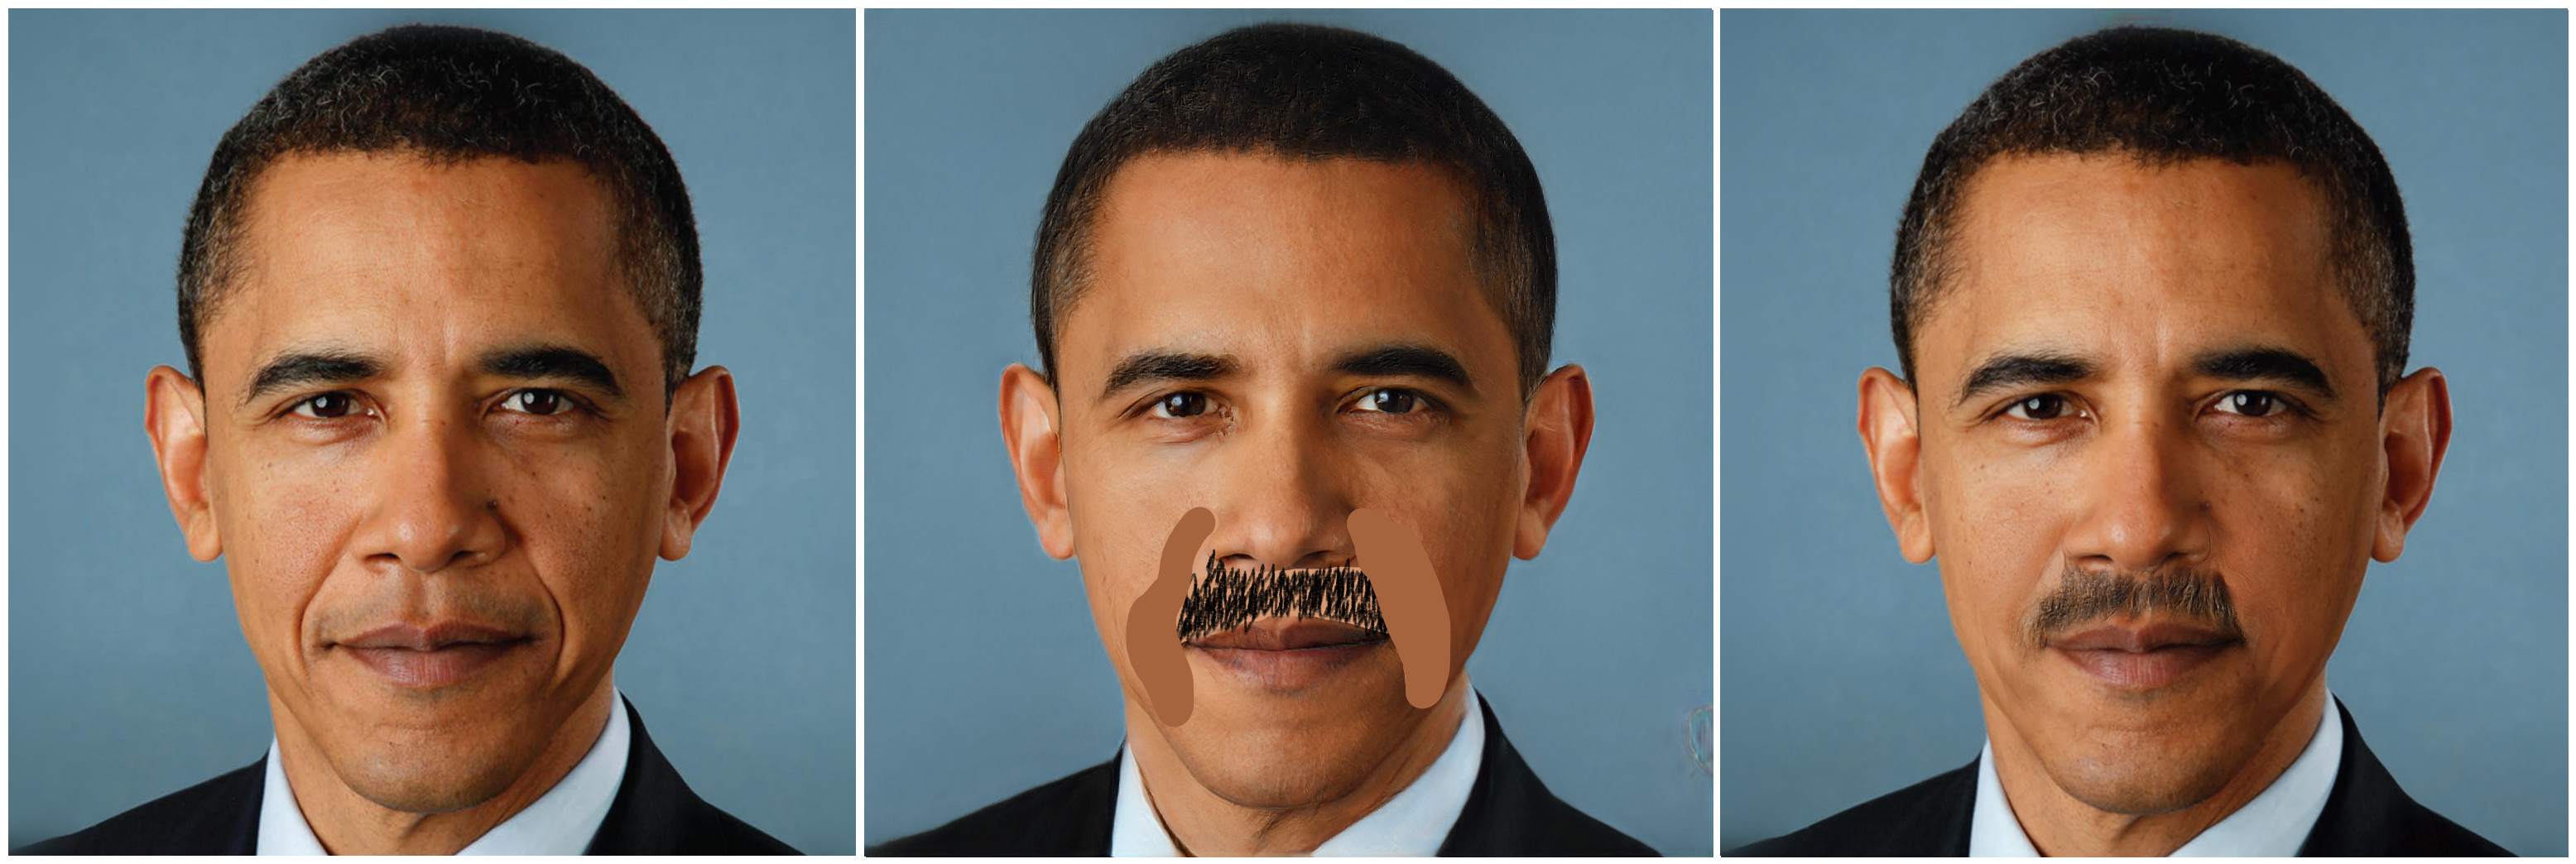
\includegraphics[width= 0.95\linewidth]{images/local_obama.jpg}
 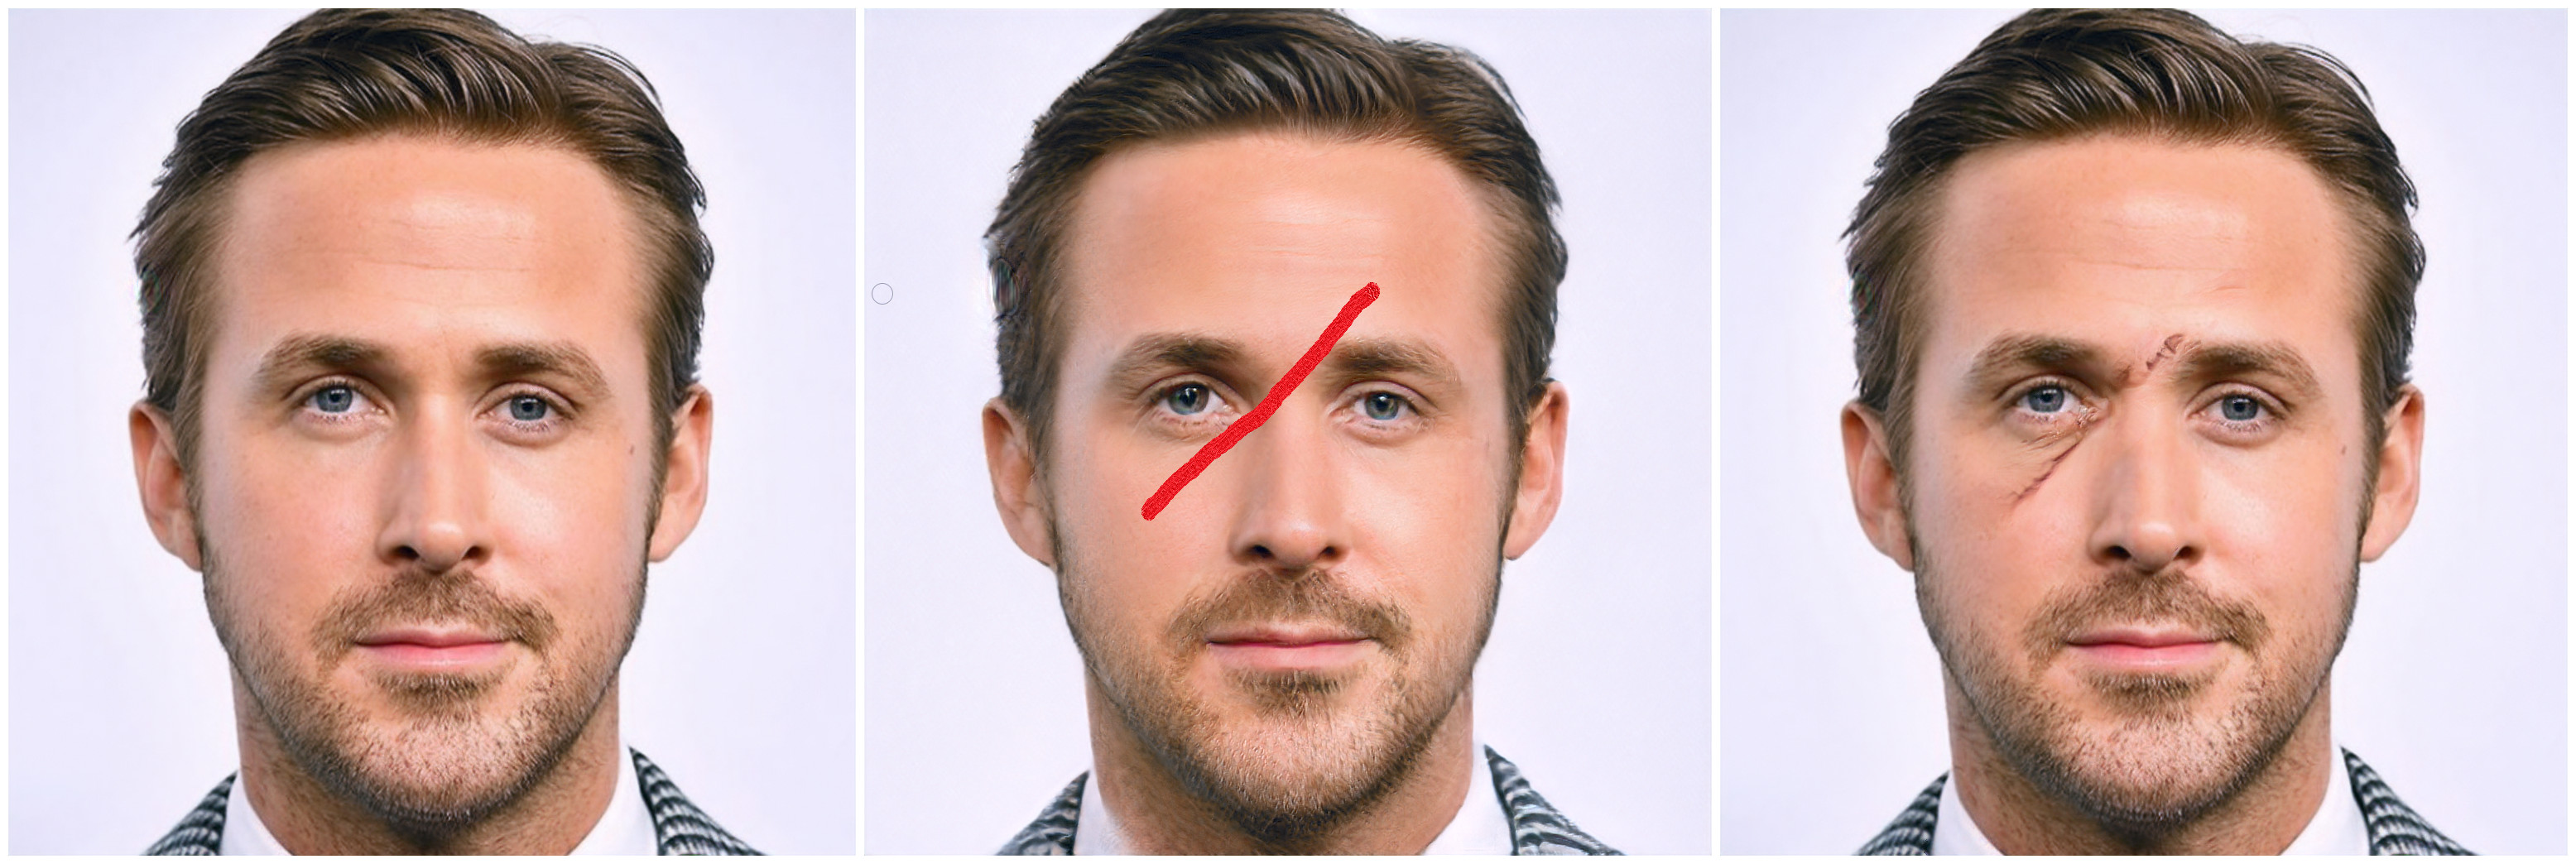
\includegraphics[width=0.95\linewidth]{images/local_ryan.jpg}
\caption{\textbf{兴趣区域编辑图解~\cite{abdal2020image2stylegan2}.} 从左到右: 基础模型; 涂鸦过的图像; 局部编辑的结果.}
\label{fig:local}
\end{figure}
}

\newcommand{\figrewrite}{
\begin{figure}[tbp]
\begin{center}
\includegraphics[width=0.95\linewidth]{images/ganrewriting}
\end{center}
\caption{\textbf{用于重写模型的复制-粘贴-上下文接口~\cite{zhu2016generative}.} 
%The first row is the user inputs and the last are corresponding model outputs. 
(a) 复制:用户使用笔刷选择一个区域包含一个有趣的对象或形状,定义目标. (b) 粘贴:用户定位和粘贴复制的对象到一个单一的目标图像. (c) 上下文:为了控制泛化,用户在几张图像中选择目标区域. (d) 编辑被应用到模型上,而不是应用到特定的图像上,这样新生成的图像就会在马头顶上有帽子. (e) 这种变化已经应用于不同类型的马和姿势.}
\label{fig:ganrewriting}
\end{figure}
}

\newcommand{\figood}{
\begin{figure}[tbp]
\begin{center}
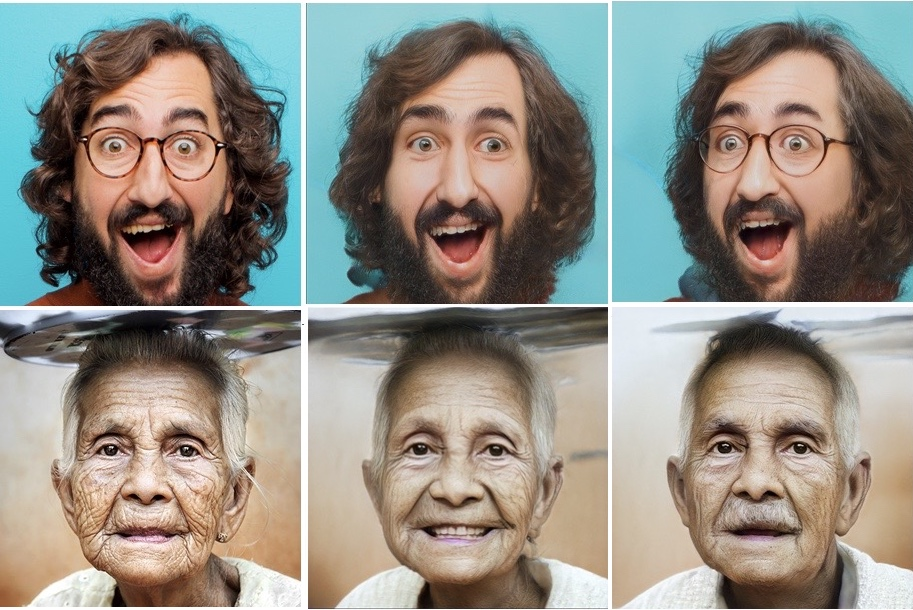
\includegraphics[width=0.95\linewidth]{images/ood}
\end{center}
\caption{\textbf{人脸图像处理的图解.} 这些是真实的图像编辑结果,来自StyleFlow~\cite{abdal2020styleflow}.}
\label{fig:ood}
\end{figure}
}

\newcommand{\figapp}{
\begin{figure}[tbp]
\begin{center}
\includegraphics[width=0.95\linewidth]{images/application_zhou}
\end{center}
\caption{\textbf{用GAN逆向进行图像处理的图解.}
GAN逆向不需要特定于任务的密集标记数据集,可以应用于许多任务,如图像重建、图像恢复和图像操作. 
% GAN inversion does not require task-specific dense-labeled datasets and can be applied to many tasks like image reconstruction (a), image restoration (b)(c)(d)(e) and image manipulation (f). 
The upper illustration (a) 来自 mGANPrior~\cite{gu2020image} 下面的(b) 来自DGP~\cite{pan2020exploiting}.}
\label{fig:application}
\end{figure}
}

\newcommand{\figcorrect}{
\begin{figure}[tbp]
\begin{center}
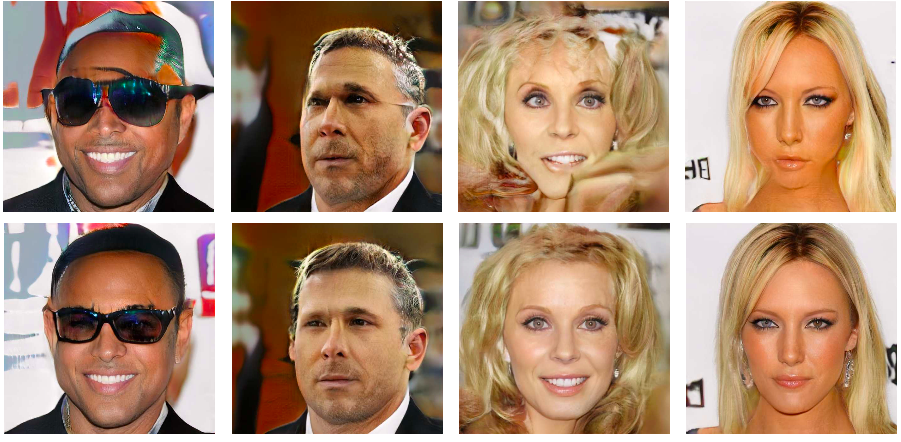
\includegraphics[width=0.98\linewidth]{images/correction}
\end{center}
\caption{\textbf{伪影校正结果.}  第一行显示的是PGGAN~\cite{karras2017progressive}生成的示例。第二行是通过将隐向量沿着正向质量方向移动而逐步修正的合成。此图来自~\cite{shen2020interpreting}.}
\label{fig:correction}
\end{figure}
}

\newcommand{\algotransfer}{
\begin{algorithm}[t]
\SetAlgoLined
\KwIn{images $x, y \in \mathbb{R}^{n \times m \times 3}$; masks $M_b$}
\KwOut{the embedded code $(\mathbf{w_o},\mathbf{n_o})$} 
$(\mathbf{w^*},\mathbf{n_i}) \leftarrow$ initialize()\;
{$\mathbf{w_o} = W_{l}(M_b,M_b,1 ,\mathbf{w^*},\mathbf{n_i},x)$\
$+ M_{st}(1-M_b,\mathbf{w^*} ,\mathbf{n_i}, y)$\;
$\mathbf{n_o} = {Mk}_{n}(M_b,\mathbf{w_o},\mathbf{n_i},x,G(\mathbf{w_o}))$\;
}
\caption{局部风格转移~\cite{abdal2020image2stylegan2}}
\label{alg:local_style_tranfer}
\end{algorithm}
}

\newcommand{\figtransfer}{
\begin{figure}[tp]
\centering
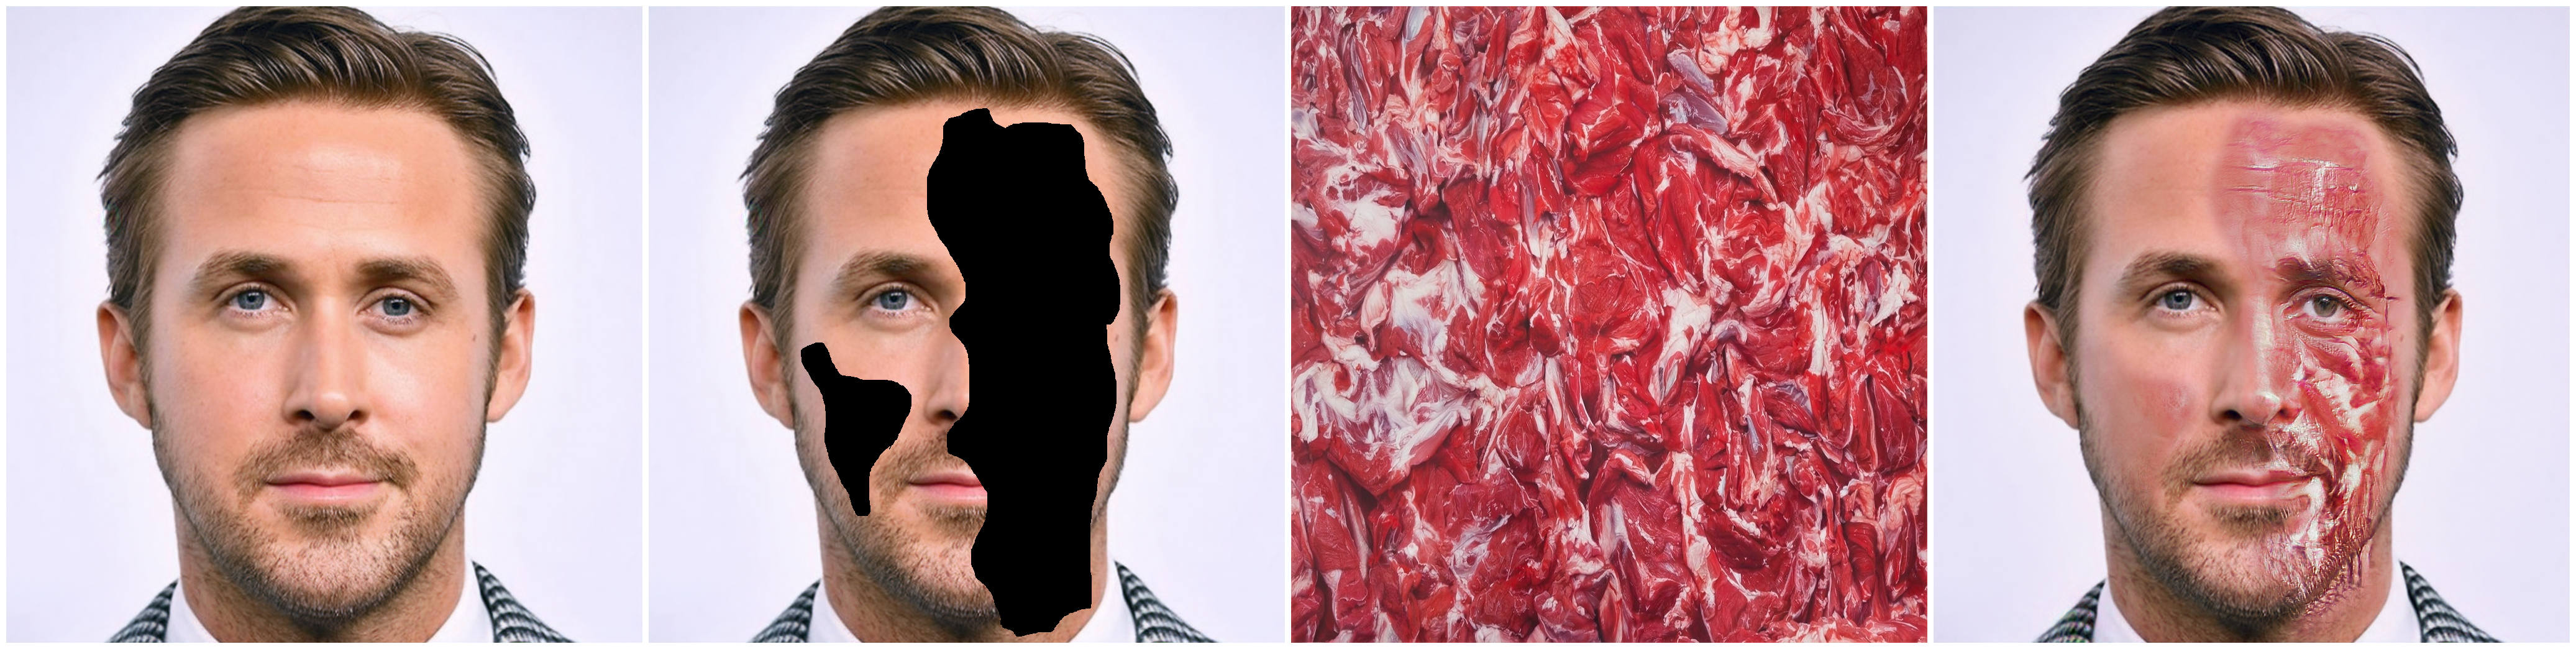
\includegraphics[width=0.95\linewidth]{images/style_ryan.jpg}
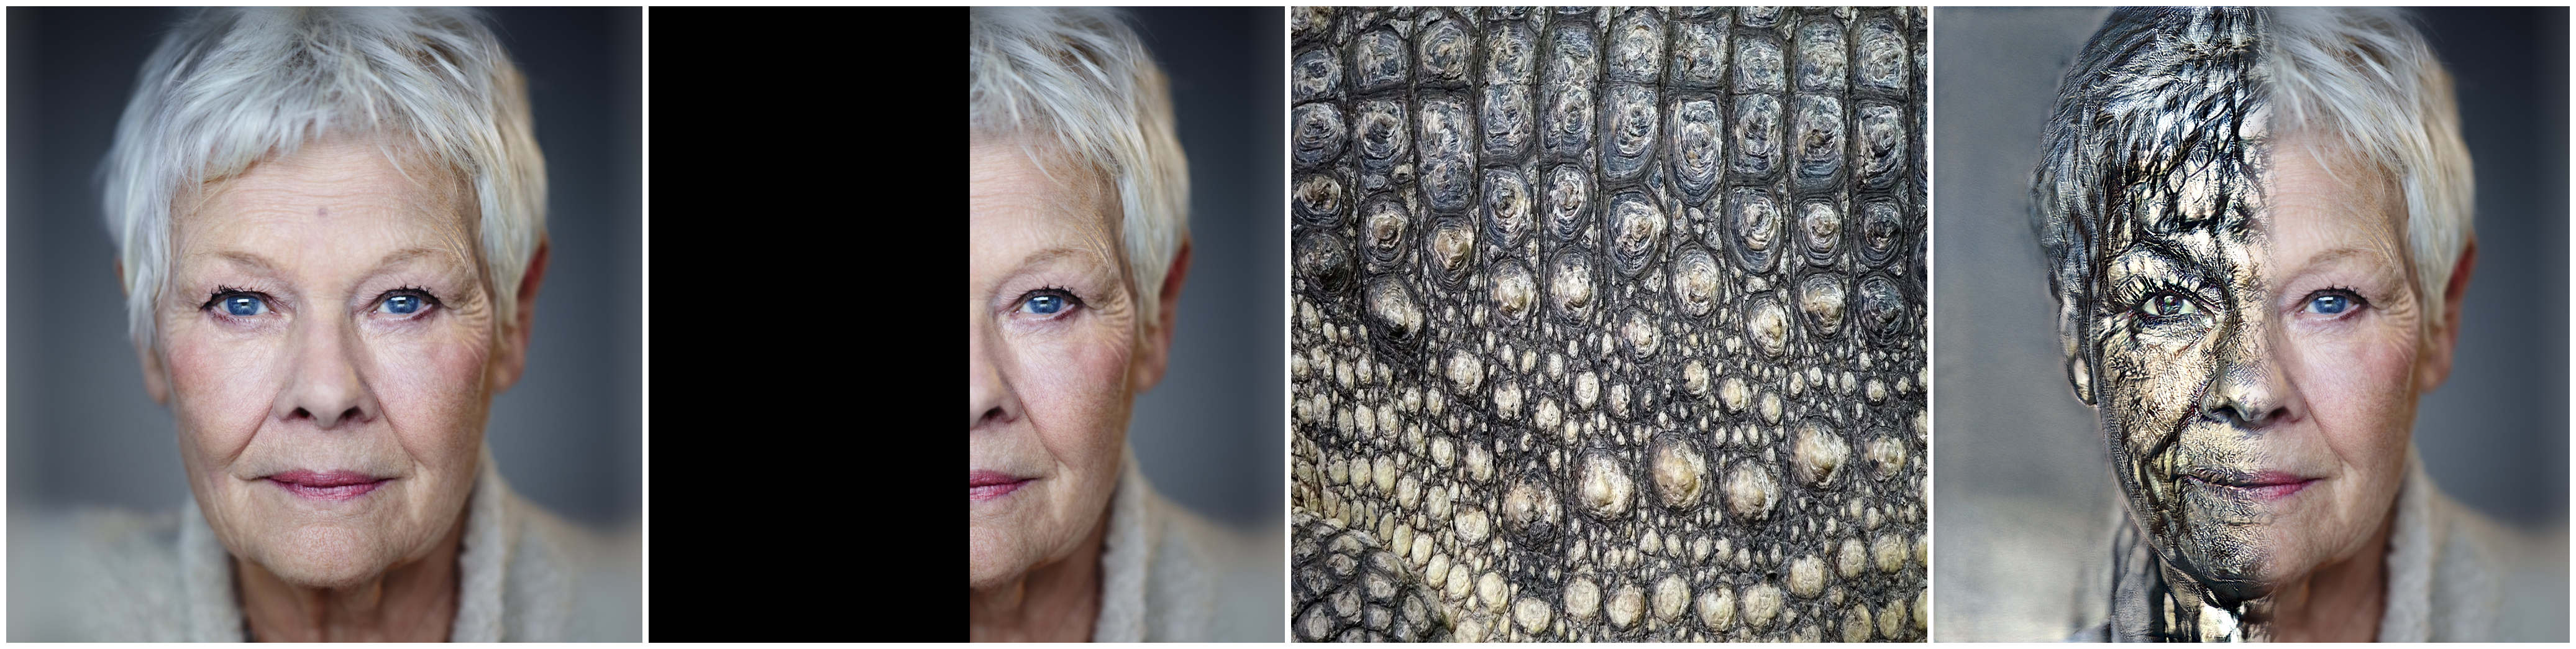
\includegraphics[width=0.95\linewidth]{images/style_judi.jpg}
\caption{\textbf{局部风格迁移图解~\cite{abdal2020image2stylegan2}.} 从左到右: 基础图像, 遮盖的区域, 风格图像, 局部风格迁移的结果.}
\label{fig:local_style_tranfer}
\end{figure}
}

\newcommand{\figinteractive}{
\begin{figure}[tbp]
\begin{center}
\includegraphics[width=0.95\linewidth]{images/interactive}
\end{center}
\caption{\textbf{使用GAN逆向进行交互式图像生成的图解.} (a) 插图结果来自 ~\cite{zhu2016generative}. 用户可以使用笔刷工具从零开始生成图像,并不断添加更多的涂鸦或草图以改进。最后一行显示了与生成的图像最相似的真实图像。虚线表示素描工具,彩色涂鸦表示颜色笔刷.
(b) 来自 GANPaint~\cite{bau2019ganpaint}. 笔刷可以绘制有语义意义的单元,如移走椅子或增加屋顶.
}
\label{fig:interactive}
\end{figure}
}

\newcommand{\figdiffusion}{
\begin{figure}[tbp]
\begin{center}
\includegraphics[width=0.95\linewidth]{images/diffusion.pdf}
\end{center}
\caption{\textbf{使用域内GAN逆向方法的语义扩散结果~\cite{zhu2020indomain}}. 第一列中的目标图像自然地扩散到第一行的上下文图像中,并保留标识.}
\label{fig:diffusion}
\end{figure}
}

\newcommand{\tabfeature}{
\begin{table*}[htbp]
\caption{逆向方法的特点. `Type' 包括基于学习的 (L.), 基于优化的(O.), 混合的(H.), 以及 封闭式的 (C.) GAN 逆向. I.-D., S.-A., L.-W., N.-I., R.-I. 和 O.-D. 分别表示发现可解释的方向(包括有监督的 (S.) 或无监督的(U.) 方式)、语义感知、逐层、非干涉的、感兴趣区域和分布外的特点. GAN模型和数据集表示哪个预训练的模型是在哪个数据集上,用哪个方法进行逆向的,这些可以在章节~\ref{sec:model_data}中找到.}
\label{tab:taxonomy}
\begin{center}
\scalebox{0.92}{
\begin{tabular}{c|c|c|c|c|c|c|c|c|c|c}
\toprule
Method  & Publication & Type &I.-D. &S.-A. &L.-W. &N.-I. &R.-I. &O.-D. &GAN Model & Dataset \\\hline
Zhu~\etal~\cite{zhu2016generative} &2016, NeurIPS &H. &\nxmark &\nxmark &\nxmark &\nxmark &\nxmark &\nxmark &\cite{radford2016dcgan} &\cite{yu2014local,zhou2014places,yu2015lsun}\\
Creswell~\etal~\cite{creswell2018inverting} &2018, TNNLS &O. &\nxmark &\nxmark &\nxmark &\nxmark &\nxmark &\nxmark &\cite{radford2016dcgan,gulrajani2017improved} &\cite{yu2014local,liu2015faceattributes}\\
GAN Dissection~\cite{bau2019gandissect} &2019, ICLR &O. &\nxmark &\ncmark &\ncmark &\nxmark &\ncmark &\nxmark &\cite{karras2017progressive} &\cite{yu2015lsun}\\
GAN Paint~\cite{bau2019ganpaint} & 2019, TOG &H. &\nxmark &\ncmark &\ncmark &\nxmark &\ncmark &\nxmark & \cite{karras2017progressive} & \cite{yu2015lsun}\\
Raj~\etal~\cite{raj2019gan} &2019, ICCV &O. &\nxmark &\nxmark &\nxmark &\nxmark &\nxmark &\nxmark &\cite{radford2016dcgan,zhang2019self} &\cite{yu2015lsun,lecun1998mnist,liu2015faceattributes}\\
GANSeeing~\cite{bau2019seeing} &2019, ICCV &H. &\nxmark &\ncmark &\ncmark &\nxmark & \nxmark &\nxmark &\cite{gulrajani2017improved,karras2017progressive,karras2019style}  &\cite{yu2015lsun}\\
Image2StyleGAN~\cite{abdal2019image2stylegan} &2019, ICCV &O. &\nxmark &\ncmark &\nxmark &\nxmark &\nxmark &\nxmark &\cite{karras2019style} &\cite{karras2019style} \\
Image2StyleGAN++~\cite{abdal2020image2stylegan2} &2020, CVPR &O. &\nxmark &\ncmark &\nxmark &\nxmark &\ncmark&\nxmark &\cite{karras2017progressive,karras2019style} &\cite{karras2017progressive,karras2019style}\\
mGANPrior~\cite{gu2020image} &2020, CVPR &O. &\nxmark &\ncmark &\ncmark &\ncmark &\nxmark &\ncmark &\cite{karras2017progressive,karras2019style} &\cite{karras2017progressive,karras2019style,yu2015lsun}\\
%IIN~\cite{esser2020invertible} &2020, CVPR &  &  &  &  &  &  &\\
Editing in Style~\cite{collins2020uncovering} &2020, CVPR &O. &\nxmark &\ncmark &\nxmark &\nxmark &\ncmark &\nxmark &\cite{karras2017progressive,karras2019style,karras2020analyzing} &\cite{karras2019style,yu2015lsun}\\
StyleRig~\cite{tewari2020stylerig} &2020, CVPR &L. &\nxmark &\ncmark &\nxmark &\nxmark &\nxmark &\nxmark &\cite{karras2019style} &\cite{karras2019style}\\
InterFaceGAN~\cite{shen2020interpreting} &2020, CVPR &L., O. &S. &\ncmark &\ncmark &\ncmark &\nxmark &\ncmark  &\cite{karras2017progressive,karras2019style} &\cite{karras2019style}\\
YLG~\cite{daras2020your} &2020, CVPR &O. &\nxmark &\nxmark &\nxmark &\nxmark &\nxmark &\ncmark &\cite{zhang2019self} &\cite{russakovsky2015imagenet}\\
GANRewriting~\cite{bau2020rewriting} &2020, ECCV &O. &\nxmark &\ncmark &\nxmark &\nxmark &\ncmark &\nxmark &\cite{karras2017progressive,karras2020analyzing} &\cite{yu2015lsun}\\
DGP~\cite{pan2020exploiting} &2020, ECCV &O. &\nxmark &\nxmark &\ncmark &\nxmark &\nxmark &\nxmark &\cite{brock2018large} &\cite{zhou2014places,russakovsky2015imagenet}\\
Huh~\etal~\cite{huh2020transforming} &2020, ECCV &O. &\nxmark &\ncmark &\nxmark &\nxmark &\ncmark &\ncmark &\cite{brock2018large,karras2020analyzing} &\cite{russakovsky2015imagenet,yu2015lsun,karras2019style}\\
IDInvert~\cite{zhu2020indomain} &2020, ECCV &H. &\nxmark &\ncmark &\nxmark &\nxmark &\nxmark &\ncmark &\cite{karras2019style}  &\cite{karras2019style,yu2015lsun}\\
StyleGAN2 Distillation~\cite{viazovetskyi2020distillation} &2020, ECCV &O. &S. &\ncmark &\nxmark &\ncmark &\nxmark &\ncmark &\cite{karras2020analyzing} &\cite{karras2019style}\\
GANSteering~\cite{jahanian2020steerability} &2020, ICLR &O. &S. &\ncmark &\nxmark &\nxmark &\nxmark &\nxmark &\cite{brock2018large,karras2019style,radford2016dcgan} &\cite{russakovsky2015imagenet,yu2015lsun,karras2019style}\\
GANLatentDiscovery~\cite{voynov2020latent} &2020, ICML &O. &U. &\ncmark &\nxmark &\nxmark &\nxmark &\nxmark &\cite{brock2018large,karras2017progressive} &\cite{karras2017progressive,jin2017towards,lecun1998mnist}\\
PIE~\cite{tewari2020pie} &2020, TOG &O. &S. &\ncmark &\nxmark &\ncmark &\nxmark &\ncmark &\cite{karras2019style}  &\cite{karras2019style}\\
StyleFlow~\cite{abdal2020styleflow} &2020, arxiv &O. &S. &\ncmark &\nxmark &\ncmark &\nxmark &\ncmark &\cite{karras2019style,karras2020analyzing}  &\cite{karras2019style,yu2015lsun}\\
GANSpace~\cite{eric2020GANSpace} &2020, arxiv &O. &U. &\ncmark &\ncmark &\ncmark &\nxmark &\nxmark &\cite{brock2018large,karras2019style,karras2020analyzing} &\cite{karras2017progressive,yu2015lsun}\\
Nitzan~\etal~\cite{nitzan2020harness} &2020, arxiv &L. &\nxmark &\ncmark &\nxmark &\ncmark &\nxmark &\nxmark &\cite{karras2019style}  &\cite{karras2017progressive,karras2019style}\\
% Li~\etal~\cite{li2020latent} &2020, arxiv &O. &\nxmark &\ncmark &\nxmark &\ncmark &\nxmark &\nxmark &\cite{gulrajani2017improved}  &\cite{xiao2017fashion,yu2017jittor}\\
SeFa~\cite{shen2020closedform} &2020, arxiv &C. &U. &\ncmark &\ncmark &\ncmark &\ncmark &\ncmark &\cite{karras2017progressive,brock2018large,karras2019style,karras2020analyzing} &\cite{naik2014streetscore,karras2017progressive,karras2019style,yu2015lsun,russakovsky2015imagenet}\\
Aberdam~\etal~\cite{aberdam2020invert} &2020, arxiv &O. &\nxmark &\nxmark &\ncmark &\nxmark &\nxmark &\nxmark & a two-layer model & \cite{lecun1998mnist} \\
StyleGAN-Encoder~\cite{guan2020faster} &2020, arxiv &L. &\nxmark &\ncmark &\nxmark &\ncmark &\nxmark &\nxmark &\cite{karras2019style} &\cite{karras2017progressive,karras2019style,chen2014cross}\\
GH-Feat~\cite{xu2020ghfeat} &2020, arxiv &L. &\nxmark &\ncmark &\ncmark &\nxmark &\nxmark &\nxmark &\cite{karras2019style} &\cite{lecun1998mnist,yu2015lsun,karras2019style}\\
pSp~\cite{richardson2020encoding} &2020, arxiv &L. &\nxmark &\ncmark &\ncmark &\ncmark &\ncmark &\ncmark &\cite{karras2020analyzing} &\cite{karras2017progressive}\\
Style Intervention~\cite{liu2020style} &2020, arxiv &O. &S. &\ncmark &\nxmark &\ncmark &\ncmark &\ncmark &\cite{karras2020analyzing} &\cite{liu2020style}\\
StyleSpace~\cite{wu2020stylespace} &2020, arxiv &O.&S. &\ncmark &\nxmark &\ncmark &\ncmark &\ncmark &\cite{karras2020analyzing} &\cite{karras2019style,yu2015lsun}\\
Lu~\etal~\cite{lu2020discovery} &2020, arxiv &L. &U. &\ncmark &\nxmark &\ncmark &\nxmark &\nxmark &\cite{karras2020analyzing,karras2017progressive,miyato2018spectral} &\cite{karras2019style,russakovsky2015imagenet}\\
Cherepkov~\etal~\cite{cherepkov2020navigating} &2020, arxiv &O. &U. &\ncmark &\nxmark &\ncmark &\nxmark &\ncmark &\cite{karras2020analyzing} &\cite{karras2019style,yu2015lsun}\\
Nurit~\etal~\cite{nurit2020steerability} &2020, arxiv &C. &U. &\ncmark &\nxmark &\ncmark &\nxmark &\nxmark &\cite{brock2018large} &\cite{russakovsky2015imagenet} \\

\bottomrule
\end{tabular}
}
\end{center}
\end{table*}
% \footnotetext[1]{They use a self-defined two-layer GAN model.}
}
% \def\eg{\emph{e.g.}}
% \def\ie{\emph{i.e.}}
% \def\etal{\emph{et al.}}
% \def\etc{\emph{etc}}
% \def\iid{\emph{i.i.d.}}
\newcommand{\eg}{\textit{e.g.}}
\newcommand{\ie}{\textit{i.e.}}
\newcommand{\etal}{\textit{et al.}}
\newcommand{\etc}{\textit{etc}}
\newcommand{\iid}{\textit{i.i.d.}}

\newcommand{\z}{\mathbf{z}}
\newcommand{\x}{\mathbf{x}} 
\newcommand{\y}{\mathbf{y}}
\newcommand{\q}{\mathbf{q}}
\newcommand{\p}{\mathbf{p}}
\newcommand{\w}{\mathbf{w}}
\newcommand{\n}{\mathbf{n}} 
\newcommand{\ww}{\boldsymbol{w}} 
\newcommand{\bb}{\mathbf{b}}
\newcommand{\rr}{\mathbf{r}}
\newcommand{\A}{\mathbf{A}} 
\newcommand{\W}{\mathbf{W}} 
\newcommand{\M}{\mathbf{M}} 
\newcommand{\PP}{\mathbf{P}}
\newcommand{\D}{\mathbf{D}} 
\newcommand{\I}{\mathbf{I}} 

\newcommand{\R}{\mathbb{R}} 
\newcommand{\E}{\mathbb{E}} 

\newcommand{\ncmark}{\ding{51}}
\newcommand{\nxmark}{\ding{55}}

\newcommand{\EDIT}[4][]{\strut{\color{#3}{\hspace{0pt}\initials{#2}{\color{red}\sout{#1}}{#4}}}}
\newcommand{\TK}[2][]{\protect\EDIT[#1]{TK}{maroon}{#2}}
\newcommand{\SL}[2][]{\protect\EDIT[#1]{SL}{olive}{#2}}
\newcommand{\TA}[2][]{\protect\EDIT[#1]{TA}{internationalkleinblue}{#2}}
\newcommand{\JL}[2][]{\protect\EDIT[#1]{JL}{red}{#2}}
\newcommand{\TODO}[2][]{\protect\EDIT[#1]{}{celestialblue}{{\sc todo} #2}}
\newcommand{\FINAL}[2][]{#2} %
\newcommand{\website}{\FINAL{\texttt{\small{\href{https://github.com/weihaox/awesome-image-translation/blob/master/awesome-gan-inversion.md}{github.com/weihaox/awesome-gan-inversion}}}}}
\usepackage{xeCJK}
\begin{document}
\title{GAN Inversion: A Survey}


\author{Weihao~Xia,
Yulun Zhang,
Yujiu~Yang*, %
Jing-Hao~Xue, %
Bolei~Zhou*,
Ming-Hsuan~Yang*%
\thanks{This work has been submitted to the IEEE for possible publication. Copyright may be transferred without notice, after which this version may no longer be accessible.}
\thanks{*Corresponding authors}
\thanks{W.~Xia and Y.~Yang are with Tsinghua Shenzhen International Graduate School, Tsinghua University, China.
Email: weihaox@outlook.com, yang.yujiu@sz.tsinghua.edu.cn}
\thanks{Y.~Zhang is with Department of Electrical and Computer Engineering, Northeastern University, USA.
Email: yulun100@gmail.com}
\thanks{J.-H.~Xue is with the Department of Statistical Science, University College London, UK.
Email: jinghao.xue@ucl.ac.uk}
\thanks{B.~Zhou is with Department of Information Engineering, The Chinese University of Hong Kong, Shatin, Hong Kong SAR, China.
Email: bzhou@ie.cuhk.edu.hk}
\thanks{M.-H.~Yang is with Electrical Engineering and Computer Science, University of California at Merced, USA.
Email: mhyang@ucmerced.edu}
}
\IEEEtitleabstractindextext{
	\begin{abstract}
		GAN逆向的目的是将给定的图像逆向回预先训练好的GAN模型的隐空间,以便生成器通过逆向的编码如实地重建图像。GAN逆向作为一种新兴的连接真实和虚假图像领域的技术,在使预先训练好的GAN模型,如StyleGAN和BigGAN,用于真实图像编辑应用中起着至关重要的作用。同时,GAN逆向也为GAN的隐空间解释性和真实图像的生成提供了思路。
		
		在本文中,我们对GAN逆向进行了概述,并重点介绍了它最近的算法和应用。我们涵盖了GAN逆向的重要技术及其在图像恢复和图像处理中的应用。
		
		我们进一步阐述了未来方向的一些趋势和挑战。在\website 上可以找到GAN逆向方法、数据集和其他相关信息的列表。 
	\end{abstract}
	
	\begin{IEEEkeywords}
		生成对抗网络, 可解释机器学习, 图像重建, 图像处理
	\end{IEEEkeywords}
}

% \tableofcontents

\maketitle
\IEEEpeerreviewmaketitle

\section{Introduction}
\label{sec:introduction}
\IEEEPARstart{}{生成对抗网络} (GAN)框架是一种深度学习架构,可以估计数据点是如何在概率框架中生成的~\cite{goodfellow2014generative,goodfellow2016deep}.
它由两个相互作用的神经网络组成: 通过对抗的过程共同训练的生成器 $G$ 和判别器$D$。
$G$的目标是合成与真实数据相思的假数据,$D$的目标是分辨真实和虚假的数据.
通过一个对抗性的训练过程,生成器$G$可以生成与真实数据分布匹配的假数据。
近年来,GANs已被应用于许多任务中
包括图像转换~\cite{mao2019mode,lee2018drit,huang2018munit}, 图像处理~\cite{wang2018high,xia2020gaze,li2020manigan} 以及图像修复~\cite{zhang2017beyond,tsai2017deep,xu2017text,ma2017learning,li2018flow}.

大量的GAN模型, 如 PGGAN~\cite{karras2017progressive}, BigGAN~\cite{brock2018large} 和StyleGAN ~\cite{karras2019style,karras2020analyzing}, 可以从随机噪声输入中合成高质量和多样性的图像. 
最近的研究表明,GAN能有效地在中间特征~\cite{bau2019semantic} 和隐空间中~\cite{goetschalckx2019ganalyze,jahanian2020steerability, shen2020interpreting}编码丰富的语义信息,作为图像生成的结果.
这些方法可以通过改变潜在代码来合成具有不同属性的图像,如老化、表情、光照方向等。
然而,由于GAN缺乏推理功能和编码器,这种对隐空间的操作只适用于GAN生成的图像,并不适用于任何给定的真实图像。

\figoverview

相比之下,GAN逆向的目标是将给定的图像逆向回预先训练好的GAN模型的隐空间。然后,图像就可以通过生成器从被逆向的编码中如实地重建出来。
由于GAN逆向在连接真实和虚假图像域方面起着至关重要的作用,因此取得了显著的进展~\cite{zhu2016generative,abdal2019image2stylegan,abdal2020image2stylegan2,bau2019seeing,karras2020analyzing,huh2020transforming,pan2020exploiting,jahanian2020steerability,shen2020interpreting}. 
GAN逆向使得在现有训练过的GAN的隐空间中发现的可控方向适用于真实的图像编辑,而不需要特别的监督或昂贵的优化。
如图~\ref{fig:overview}, 将真实图像逆向到隐空间后,我们可以沿着一个特定的方向改变其编码,编辑图像的相应属性。
GAN逆向作为一个将生成对抗网络与可解释机器学习技术相结合的快速发展的领域,不仅提供了一种灵活的替代图像编辑框架,而且有助于揭示深度生成模型的内在机制。

在这篇文章中,我们提出了一个全面的调查GAN逆向方法,重点是算法和应用。据我们所知,这项工作是对快速增长的GAN逆向的第一次调查,并有以下贡献。首先,我们对在GAN逆向的所有方面的层次和结构,提供了一个全面和系统的回顾,以及深刻的分析。其次,我们对GAN逆向方法的性质和性能进行了比较总结。第三,我们讨论了挑战和有待解决的问题,并确定了未来研究的趋势。

\section{Preliminaries}
\label{sec:overview}

\subsection{翻译的术语表}
\label{sec:term}
inversion 逆向;
entangle 耦合的;
disentangle 解耦的;
transform 变换;
reconstruction 重建或者重构;
latent code 隐编码或者隐向量;
latent space 隐空间;
style 风格;

\subsection{问题定义}
\label{sec:definition}
无条件GAN的生成器学习映射 $G: \mathcal{Z} \to \mathcal{X}$. 
当 $\z_1, \z_2 \in \mathcal{Z}$ 在$\mathcal{Z}$ 空间中是接近的, 相应的图片$x_1, x_2 \in \mathcal{X}$ 在视觉上接近. 
生成器的逆向是将数据 $x$ 逆映射到隐表示$\z^*$, 或者等价地, 找到一个图像${x^*}$ ,该图像可以被一个训练好的生成器$G$完全合成,并且与真实图片$x$接近.
把逆变换的信号定义为 $x \in \R^{n}$, 训练好的生成器定义为$G: \R^{n_{0}} \to \R^{n}$, 隐向量定义为$\z \in \R^{n_{0}}$, 我们研究以下逆向问题:
\begin{equation}
\z^*=\underset{\z}{\arg \min } \ \ell(G(\z), x),
\label{eqn:def}
\end{equation}
其中 $\ell(\cdot)$ 是一个在图像或特征空间中的距离度量, 假设 $G$ 是一个前馈神经网络. 
一般的, $\ell(\cdot)$ 基于$\ell_1$, $\ell_2$, 感知度量 ~\cite{johnson2016perceptual}, 和 LPIPS~\cite{zhang2018unreasonable} 度量.
由于$G(\z)$的非凸性,这通常是一个非凸问题,而GAN逆向方法的重点是重建图像内容。

\subsection{预训练的GAN模型和数据集}
\label{sec:model_data}
深度生成模型,如GAN ~\cite{goodfellow2014generative} 已被用于模拟自然图像分布和合成照片真实感图像。 gan的最新进展,如DCGAN ~\cite{radford2016dcgan}, WGAN~\cite{gulrajani2017improved}, PGGAN~\cite{karras2017progressive}, BigGAN~\cite{brock2018large}, StyleGAN~\cite{karras2019style} 以及 StyleGAN2~\cite{karras2020analyzing} 开发了更好的架构、损失和训练方法. 这些模型是在不同的数据集上训练的,包括人脸 (CelebA-HQ~\cite{karras2017progressive}, FFHQ~\cite{karras2019style,karras2020analyzing}, AnimeFaces~\cite{jin2017towards} 和 AnimalFace~\cite{liu2019funit}), 场景 (LSUN~\cite{yu2015lsun}), 和目标 (LSUN~\cite{yu2015lsun} 以及imagenet~\cite{russakovsky2015imagenet}).

\subsubsection{GAN 模型} 
\label{sec:gan models}

\noindent\textbf{DCGAN}~\cite{radford2016dcgan} 在鉴别器中使用卷积,在生成器中使用反卷积. \par

\vspace{1mm}
\noindent\textbf{WGAN}~\cite{gulrajani2017improved} 最小化生成的数据分布和真实数据分布之间的Wasserstein距离,这提供了更多的模型稳定性,使训练过程更容易.\par

\vspace{1mm}
\noindent\textbf{PGGAN}~\cite{karras2017progressive}, 也被称为ProGAN或Progressive GAN,在训练过程中使用一种渐进式策略. 
关键的思想是,从生成器和鉴别器的低分辨率开始,然后添加新的层,随着训练的进行,这些层对越来越细粒度的细节进行建模. 
这提高了训练速度和稳定性,从而促进图像合成在更高的分辨率, \eg, $1024 \times 1024$ 像素的CelebA 图像. \par

\vspace{1mm}
\noindent\textbf{BigGAN}~\cite{brock2018large} 生成高分辨率和高质量的图像,通过修改放大、架构变化和正交正则化来提高大规模GAN的可伸缩性、鲁棒性和稳定性.\par

\vspace{1mm}
\noindent\textbf{StyleGAN}~\cite{karras2019style} 隐式地学习分层潜在风格的图像生成。. 
这个模型操纵每个通道的平均值和方差来有效控制图像的风格~\cite{huang2017adain} .
StyleGAN生成器将风格向量(由映射网络定义)和随机变化(由噪声层提供)作为输入,而不是来自隐空间的样本,来生成合成图像. 
这提供了在不同细节级别上控制生成图像的样式.
StyleGAN2 模型~\cite{karras2020analyzing} 通过提出权值解调、路径长度正则化、重新设计生成器和去除渐进增长,进一步改善图像质量. 
基于StyleGAN的架构已经应用于许多应用场景~\cite{gabbay2019style,zhu2020sean,zhu2020semantically}.\par

\subsubsection{数据集}
\label{sec:datasets}

\vspace{1mm}
\noindent\textbf{ImageNet}~\cite{russakovsky2015imagenet} 是一个大规模的手工标注的数据集,用于视觉对象识别研究,包含超过1400万幅图像,超过20000个类别.\par

\vspace{1mm}
\noindent\textbf{CelebA}~\cite{liu2015faceattributes} 是一个大型的人脸属性数据集,由200K张名人图像组成,每张图像有40个属性标注。CelebA,以及后来的CelebA-HQ~\cite{karras2017progressive}, CelebAMask-HQ~\cite{CelebAMask-HQ}, 以及 CelebA-Spoof~\cite{CelebA-Spoof}, 广泛应用于人脸图像的生成和处理.\par

\vspace{1mm}
\noindent\textbf{Flickr-Faces-HQ} (FFHQ)~\cite{karras2019style,karras2020analyzing} 是一个从Flickr抓取的高质量人脸图像数据集,它包含70,000张$1024 \times 1024$像素的高质量人脸图像,在年龄、种族和图像背景方面有相当大的差异。\par

\vspace{1mm}
\noindent\textbf{LSUN}~\cite{yu2015lsun} 包含10个场景类别(例如,卧室,教堂,或塔)和20个对象类别的大约100万个标签图像 (例如,鸟、猫或公共汽车).
教堂和卧室场景图像、汽车和鸟类物体图像经常被用在GAN逆向问题研究中.\par

此外,一些GAN逆向研究在他们的实验中也使用了其他数据集~\cite{lecun1998mnist,xiao2017fashion,krizhevsky2009learning,chen2014cross,yu2017jittor,xia2020tedigan}, 比如 \textbf{DeepFashion}~\cite{liu2016fashion, liu2016deepfashion, Ge2019DeepFashion2}, \textbf{AnimeFaces}~\cite{jin2017towards}, 以及 \textbf{StreetScapes}~\cite{naik2014streetscore}.

\subsection{评价指标}
\label{sec:metrics}

基于GANs的图像合成通常在摄影真实感、多样性、可解释性和可解耦方面进行评价。通常采用结构相似度(PSNR和SSIM)和感知质量(IQA方法)来衡量照片真实性。多样性对GAN的生成方法尤为重要;最广泛使用的度量标准是IS、FID和LPIPS;最近的研究也使用SWD。可解释性和可解耦性是GAN逆向任务中最相关的指标。
在文献中,有一些方法~\cite{nitzan2020harness} 使用余弦距离或欧氏距离来评估输入和输出之间的不同属性, 而其他人~\cite{voynov2020latent} 使用分类准确性进行评估.

\subsubsection{图象质量评价}
\label{sec:iqa}

\noindent\textbf{Mean Opinion Score} (MOS) 以及 \textbf{Difference Mean Opinion Score} (DMOS) 已经被用于主观的图像质量评估,即要求人类评分者给图像的感知质量打分.
通常,分数从 $1$ (不好) 到 $5$ (好), 最后的MOS值是所有评分的算术平均值.
然而,这个指标也有缺点, 比如, 非线性的感知比例、偏差和方差。



\vspace{1mm}
\noindent\textbf{Peak Signal-to-Noise Ratio} (PSNR) 是衡量重建质量最广泛使用的标准之一.
真实图像 $I$ 与重建图像 $\hat{I}$ 之间的PSNR 定义为图像最概然像素值(表示为$L$)和均方误差图像间 (MSE) :
\begin{align}
{\rm PSNR} &= 10 \cdot \log_{10} (\frac {L^2} {\frac{1}{N} \sum_{i=1}^{N} (I(i) - \hat{I}(i))^2}),
\label{eqn:mse}
\end{align}
如果使用$n$比特的线性脉冲编码调制表示, $L$ 等于$2^{n}-1$, 比如, 一般情况下$255$使用8位比特表示,即$n=8,L=255$.

\vspace{1mm}
\noindent\textbf{Structural Similarity} (SSIM)~\cite{TIP2004ImageWang} 基于亮度、对比度和结构方面的独立性比较来衡量图像之间的结构相似性.
带有 $N$ 个像素的两个图片$I$ 和 $\hat{I}$ 的SSIM为:
\begin{equation}
\label{eqn:ssim}
{\rm SSIM}(I, \hat{I}) = [\mathcal{C}_l(I, \hat{I})]^\alpha
                         [\mathcal{C}_c(I, \hat{I})]^\beta
                         [\mathcal{C}_s(I, \hat{I})]^\gamma,
\end{equation}
其中 $\alpha$, $\beta$, $\gamma$是调整相对重要性的控制参数.
这些条款的细节可以参考~\cite{TIP2004ImageWang}.






\subsubsection{基于学习的感知质量}
\noindent\textbf{Inception Score} (IS)~\cite{salimans2016improved} 是一种广泛使用的度量标准,用于衡量由GAN模型生成的图像的质量和多样性。当给定生成的图片时,它计算在ImageNet~\cite{deng2009imagenet}上预训练的Inception-v3网络的统计信息~\cite{szegedy2016rethinking}:
\begin{equation}
\mathrm{IS} = \exp{\big (\E_{x \sim p_g} D_{KL} (p(y|x) \;\|\; p(y))\big)},
\end{equation}
其中 $x \sim p_g$ 表示$x$ 是一张采样自$p_g$的图片, $D_{KL}(p\|q)$ 是 分布$p$ 和 $q$之间的KL散度, $p(y|x)$ 是条件分布, $p(y) = \int_x p(y|x)p_g(x)$ 是边缘分布.\par

\vspace{1mm}
\noindent\textbf{Fr$\acute{e}$chet Inception Distance}~\cite{heusel2017gans} (FID) 是用在两个多元高斯分布之间的 Fr$\acute{e}$chet 距离定义的:
\begin{equation}
\mathrm{FID}=\|\mu_{r}-\mu_{g}\|^{2}+\operatorname{Tr}(\Sigma_{r}+\Sigma_{g}-2(\Sigma_{r} \Sigma_{g})^{\frac{1}{2}}),
\end{equation}
其中 $X_{r} \sim \mathcal{N}(\mu_{r}, \Sigma_{r})$ 和 $X_{g} \sim \mathcal{N}(\mu_{g}, \Sigma_{g})$ 分别为真实样本和生成样本经过Inception-v3的pool3层的2048维激活向量~\cite{szegedy2016rethinking}. 
最低的FID表示最多的感知结果.\par

\vspace{1mm}
\noindent\textbf{Fr$\acute{e}$chet Segmentation Distance} (FSD)~\cite{bau2019seeing}和FID度量的可解释:
\begin{equation}
\mathrm{FSD} = \|\mu_{g}-\mu_{t}\|^{2}+\operatorname{Tr}(\Sigma_{g}+\Sigma_{t}-2(\Sigma_{g} \Sigma_{t})^{\frac{1}{2}}),
\end{equation}
其中 $\mu_{t}$ 是训练图像样本上每个对象类的平均像素数,  $\Sigma_{t}$ 是协方差.\par

\vspace{1mm}
\noindent\textbf{Sliced Wasserstein Discrepancy} (SWD)~\cite{rabin2011wasserstein} 旨在捕获任务特定分类器输出之间的不相似性,可以通过计算投影点云的一维Wasserstein 距离来获得:
\begin{equation}
\tilde{W}(X, Y)^{2}=\int_{\theta \in \Omega} W\left(X_{\theta}, Y_{\theta}\right)^{2} \mathrm{~d} \theta
\end{equation}
其中 $X_{\theta}=\left\{\left\langle X_{i}, \theta\right\rangle\right\}_{i \in I} \subset \R$ 以及$\Omega=\left\{\theta \in \R^{d} \backslash\|\theta\|=1\right\}$ 是单位球. 
它为检测远离源支持的目标样本提供了有几何意义的指导,并以端到端可训练的方式实现有效的分布对齐.\par

\vspace{1mm}
\noindent\textbf{Learned Perceptual Image Patch Similarity} (LPIPS)~\cite{zhang2018unreasonable} 可以测量图像的感知质量,同时减少人工干预.
在给定不同网络的卷积层数的情况下,利用信道维数的余弦距离和空间维数的平均值,在两个patch之间进行计算.
为了得到网络$\mathcal{F}$参考点和扭曲点之间的距离 ${x,x_0}$ ,它首先计算层$l$的深度嵌入 , 记为 $\hat{y}^l, \hat{y}_0^l \in \R^{H_l\times W_l\times C_l}$, 正则化在通道维度中的激活, 按矢量$w^l \in \R^{C_l}$缩放每个通道并计算$\ell_2$ 距离(使用$w_l=1, \forall l$,相当于计算余弦距离):
\begin{equation}
d(x,x_0) = \sum_l \dfrac{1}{H_l W_l} \sum_{h,w} || w_l \odot ( \hat{y}_{hw}^l - \hat{y}_{0hw}^l ) ||_2^2.
\label{eqn:dist}
\end{equation}\par

\vspace{1mm}
\noindent\textbf{Perceptual Path Length} (PPL)~\cite{karras2019style} 利用VGG16~\cite{simonyan2014very}嵌入,测量两个输入之间插值的差异,通过移动后的图像与合成图像之间的两两图像距离来计算.
具体来说,将一个隐空间插值路径细分为线段,这条线段的感知总长度可以定义为每个线段的感知差的和.
隐空间 $\mathcal{Z}$中的PPL 为 
\begin{equation}
l_{\mathcal{Z}} = \E\Big[{\displaystyle\frac{1}{\epsilon^2}}d\big(G(\mathrm{slerp}({\z}_1,{\z}_2;\,t)), G(\mathrm{slerp}({\z}_1,{\z}_2;\,t+\epsilon))\big)\Big],
\end{equation}
其中 \mbox{${\z}_1,\z_2\sim P(\z),t\sim U(0,1)$}, $\epsilon$是一个小的扰动, $G$ 生成器 (比如, stylegan的生成器$g \circ f$ ),  $d(\cdot,\cdot)$ 评估产生的图像之间的感知距离. 
 $\mathcal{W}$中的PPL 以类似的方式定义:
\begin{equation}
\begin{aligned}
l_{\mathcal{Z}} = \E\Big[{\displaystyle\frac{1}{\epsilon^2}}d\big(&g(\mathrm{lerp}(f(\z_1),f(\z_2);\,t)), \\
&g(\mathrm{lerp}(f(\z_1),f(\z_2);\,t+\epsilon))\big)\Big].
\end{aligned}
\end{equation}
通常, $\mathcal{Z}$中 $\mathrm{slerp}(\cdot)$ 表示球面插值~\cite{shoemake1985animating}, 这是在归一化输入隐空间中插值最合适的方法~\cite{white2016sampling}.
 $\mathcal{W}$中用线性插值 $\mathrm{lerp}(\cdot)$, 因为$\mathcal{W}$中的向量没有以任何方式正则化。

\subsubsection{逆向准确率}
\noindent\textbf{分类精度.}
Voynov~\etal~\cite{voynov2020latent} 提出 \textbf{Reconstructor Classification Accuracy} (RCA) 通过预测给定图像变换在隐空间中产生的方向来衡量模型的可解释性。
该方法解决了多类分类问题,RCA值高意味着方向易于区分, 例如,相应的图像变换不会“干涉”或影响变化的不同因素.
Abdal~\etal~\cite{abdal2020styleflow} 使用 \textbf{Face Identity} 来评价编辑的质量,量化编辑的恒等性. 
一种人脸分类器模型~\cite{Geitgey2020Fr} 用于获取图像的嵌入,可以进行对比(编辑前后), 例如, $i_1$ 和 $i_2$, 然后计算嵌入之间的欧氏距离和余弦相似度.\par

\vspace{1mm}
\noindent\textbf{重建距离.}
Nitzan~\etal~\cite{nitzan2020harness}利用余弦相似度度量来比较表情留存的精度,其计算方法为$I_{attr}$和$I_{out}$~\cite{dlib2009}的二维地标之间的欧氏距离. 而位姿保持计算为$I_{attr}$和$I_{out}$的欧拉角之间的欧氏距离.
Abdal~\etal~\cite{abdal2020styleflow} 开发了 \textbf{Edit Consistency Score},在使用属性分类器进行分类时,基于编辑的不同排列会导致相同属性的假设,测量编辑图像之间的一致性.
例如,对表情和姿势进行编辑后得到的姿势属性,与对相同的姿势和灯光进行编辑后得到的姿势属性,期望是相同的, 在 $|\mathcal{A}_p(E_p(E_e(I))-\mathcal{A}_p(E_l(E_p(I))|$分数的约束下, 其中$E_x$表示沿着属性规范$x$进行条件编辑,$\mathcal{A}_p$表示由属性分类器回归的姿态属性向量。
\section{GAN的隐空间}
\label{sec:feature}
在介绍GAN逆向方法之前,我们首先回顾隐空间有趣的特征,比如, StyleGAN~\cite{karras2019style}的$\mathcal{W}$ 以及 $\mathcal{Z}$ 空间.
我们将会讨论GAN模型在可解释性、解耦性和可逆性方面可以学到什么.


\subsection{$\mathcal{Z}$ 空间和$\mathcal{W}$空间}
\label{sec:space}

GAN体系结构中的生成模型学习将从简单分布(例如,正态或均匀分布)中采样的值映射到生成的图像.
从分布中\emph{直接}采样的这些值形成了通常被称为隐空间$\mathcal{Z}$的结构,这些值是隐向量或隐表示,由$\z \in \mathcal{Z}$表示.
GAN的大多数隐空间可以用$\mathcal{Z}$空间来描述, 包括 DCGAN~\cite{radford2016dcgan}, PGGAN~\cite{karras2017progressive} 以及 BigGAN~\cite{brock2018large}.
和部分~\ref{sec:gan models}讨论的一样,最近的工作~\cite{karras2019style} 通过一个由$8$层的多层感知器(MLP)实现的非线性映射网络$f$,进一步将原生的$\z$转换为被映射的风格向量$\w$,形成另一个称为$\ mathcal{w}$空间的中间隐空间。. 
比如StyleGAN~\cite{karras2019style}的 $\mathcal{W}$空间, 以及StyleGAN2~\cite{karras2020analyzing}的$\mathcal{W}^{+}$ 空间 .


由于映射网络和仿射变换, StyleGAN 的 $\mathcal{W}$空间相比 $\mathcal{Z}$ 空间包含更多的解耦特征. 
$\mathcal{W}$ 空间减轻了耦合问题~\cite{karras2019style} 以便图像可以被更加方便的生成. 
其他研究也分析了$\mathcal{W}$和$\mathcal{Z}$空间的可分性和语义.
比如, Shen~\etal~\cite{shen2020interpreting} 说明使用$\mathcal{W}$空间的模型在可分性和表示方面比基于$\mathcal{Z}$空间的模型表现更好。
StyleGAN方法的生成器$G$倾向于根据$\mathcal{W}$空间学习语义信息,并且比使用$\mathcal{Z}$空间的生成器性能更好.
在语义方面,他们根据不同属性的潜在分离边界来评估分类的准确性.
使用$\mathcal{W}$空格的StyleGAN比使用$\mathcal{Z}$空间的PGGAN获得更高的精度。
$\mathcal{Z}$空间服从正态分布的约束限制了其语义属性的代表能力,因为假设可能不成立. 
为了解决基于样式生成器的内在复杂性引起的空间耦合问题s~\cite{karras2019style} 以及AdaIN正则化的空间不变性~\cite{huang2017adain}, 最新方法~\cite{liu2020style,wu2020stylespace} 进一步提出了$\mathcal{S}$ 空间来从语义层面实现空间维度上的空间解耦.
通过直接介入分割代码 $s \in \mathcal{S}$, 两个方法~\cite{liu2020style,wu2020stylespace} 都可以实现对局部变换的细粒度控制.

\subsection{可解释性}
基于网络修改、特征可视化和向量算法三组方法,已经开发出许多方法来解释隐藏的特征向量或深度模型中的单个神经元.
第一组方法侧重于修改网络架构或训练损失,以分析模型如何执行. 
Tao~\etal~\cite{Tao18attngan} 和 Li~\etal~\cite{li2019control,li2020manigan} 利用注意机制学习图像-文本匹配,通过将细粒度词级信息与中间特征映射关联,增强了在自然语言描述指导下的详细属性修改.
Xia~\etal~\cite{xia2020gaze} 引入一种多分支控制器,分别编辑头部姿态、凝视方向等辅助面部属性,实现凝视重定向和插值.

现有的方法主要集中在第二组方法,使用特征可视化来解释模型性能. 
Nguyen~\etal~\cite{nguyen2016synthesizing}对训练后从隐藏层重建图像的生成器网络的输入代码进行优化. 
近期, Daras~\etal~\cite{daras2020your} 为生成模型引入二维局部注意机制,并表明新引入的注意头确实通过可视化注意力特征图捕捉到真实图像的有趣方面.
第三组方法利用向量算术性质. 
Radford~\etal~\cite{radford2016dcgan} 展示了训练过的GAN丰富的线性结构,表明在隐空间中的代数操作可以导致在图像空间中进行有语义意义的操作. 
人们已经开发了许多方法,通过改变隐向量来合成不同的结果. 
后来的研究~\cite{bau2019inverting,shen2020interpreting,zhu2020indomain} 进一步证明了GAN的隐空间编码了丰富的层次语义信息.
这种矢量算术性质通常是通过将隐训练向特定方向$\z^{\prime}=\z+\alpha \n$移动来实现的, 其中 $\n \in \R^{d}$ 表示与特定属性对应的方向,$\alpha$是步长.

\subsection{解耦性}
\label{sec:disentanglability}

由于没有精确的定义,我们把可解耦性定义为隐向量$\z$可以被分割成不同的独立的表示部分$\mathbf{z_k}$的性质 . 
另外, \textit{多样性} 意味着每个因子$\mathbf{z_k}$ 代表一个特定的可解释的概念, 并且 \textit{独立性} 表示可以独立地分析和修改不同的因子$\mathbf{z_k}$.
这意味着对它们的联合密度进行因式分解 $p(\mathbf{\tilde{z}})=\prod_{k=0}^{K} p(\mathbf{{z}_{k}})$.
不同类别的特征很好地分离出来后,对应的潜在特征可以通过t-SNE方法~\cite{maaten2008visualizing}被可视化. 
解耦表示学习提供了一种可利用的结构,使我们能够仅改变底层状态的一些属性,例如面部图像的头发颜色,而保留所有其他属性不变。许多最近的解耦方法都是为了在训练中学习一种具有明确约束的可解释和可迁移的表示. 
比如, Liu~\etal~\cite{liu2018unified} 提出一个统一的模型,学习用于跨多个领域描述和操作数据的解耦表示, 
Lu~\etal~\cite{lu2019unsupervised} 从模糊图像中解耦地提取内容和模糊特征,进行图像复原. 

一些无条件的图像生成模型~\cite{karras2019style,karras2020analyzing} 也表现出良好的解耦性质. 
这些方法引入了一个非线性映射网络到生成器,而不是学习带有显式约束的解耦隐空间: $f:\mathcal{Z} \to \mathcal{W}$. 
比如, StyleGAN的中间隐空间 $\mathcal{W}$ ~\cite{karras2019style} 是由一个学习的分段连续映射推理而来的。在一个无监督设置中(比如,变化的因素事先不知道),它产生较少的耦合表示.
在随后的部分中,我们将展示这个很好地解耦的隐空间提供了可行的逆向并获得更好的结果.

\subsection{可逆性}
\label{sec:invertibility}
如部分~\ref{sec:space}所述, Radford~\etal~\cite{radford2016dcgan} 给出了隐表示$\z$的向量算术性质 .
Creswell~\etal~\cite{creswell2018inverting} 提出了逆向的概念及其逆向算法. 
Esser~\etal~\cite{esser2020invertible} 表明从简单分布(例如,高斯分布)中采样,有利于训练用于图像生成的生成模型。由于高斯密度的凸性,表示之间的线性操作是有意义的,线性插值可以沿着GAN的潜在空间遍历. 
 
尽管上述方法在经验上取得了良好的效果,但在理论理解模型可逆性方面却收效甚微. 
最近的方法旨在从不同的理论角度解决这一问题,例如压缩感知~\cite{bora2017sensing, gilbert2017invert, ma2018invertibility} 和稀疏表示~\cite{aberdam2020invert}.
例如, Hand~\etal~\cite{hand2020global} 建立权重服从高斯分布的全连通生成网络,只要给出其最后一层的压缩线性观测值,就能被逆向.
Gilbert~\etal~\cite{gilbert2017invert} 研究一个具有特殊激活函数的$1$层网络 (本质上是线性的concatenated ReLU~\cite{shang2016understanding}) 并且对隐向量进行了强$k$-稀疏性假设.
Ma~\etal~\cite{ma2018invertibility} 证明了由两层转置卷积和 ReLU~\cite{nair2010rectified} 激活函数组成的扩展网络是可逆的.
Aberdam~\etal~\cite{aberdam2020invert} 为一般的非统计权重矩阵提供可逆性和唯一性保证. 
In~\cite{aberdam2020invert}, 从稀疏表示理论推导出理论条件. 
它通过确保在~\eqref{eqn:def}中定义的逆向问题的解的唯一性,提供了深层生成模型的可逆性. 
一个推论是,层之间被一个因子扩展的非零元素的数量至少$2$,以确保逆向问题的唯一全局最小值,这有效地预测生成过程是否可逆.

\tabfeature
\section{GAN Inversion Methods}
\label{sec:model}



\subsection{逆向方法}
\label{sec:techniques}
主要有三种主要的GAN逆向技术来将图像投射到隐空间:基于学习的、基于优化的和混合的, 如图~\ref{fig:inversion_types}.
学习到的逆表示还具有其他特征,例如,可解释方向、语义感知、逐层、非干预的、感兴趣区域和分布外. 
表~\ref{tab:taxonomy} 列出了现有的最先进的GAN逆向方法的特点.

\figtype

\subsubsection{基于学习的GAN逆向}
\label{sec:learning-based}
基于学习的 GAN 逆向~\cite{perarnau2016invertible,zhu2016generative,bau2019inverting} 通常涉及训练一个编码网络$E(x; \theta_E)$映射图像$x$到隐向量$\z$:

\begin{equation}
\theta_E^* = \underset{\theta_E}{\arg\min} \sum_{n} \mathcal{L} (G(E(x_n; \theta_E)), \,x_n),
\label{eqn:rec_train}
\end{equation}
其中 $x_n$ 表示数据集中第$n$个图像.
预测模型$E$的架构通常等同于对抗网络的鉴别器$D$的架构,仅在最后一层有所变化.
~\eqref{eqn:rec_train}的目标是让人联想到一个自动编码器管道,包含一个编码器$E$和一个解码器$G$。在整个训练过程中,解码器$G$是固定的.
尽管~\eqref{eqn:def}中优化问题和~\eqref{eqn:rec_train}学习目标医院, 基于学习的方法通常比直接优化获得更好的性能,并且不会陷入局部最优~\cite{zhu2016generative,aberdam2020invert}.

比如, Perarnau~\etal~\cite{perarnau2016invertible} 提出了可逆性条件GAN(ICGAN)方法,将图像$x$用隐向量形式$\z$和属性向量$y$表示,通过改变$y$可以生成修改后的图像$x^{\prime}$。这种方法包括用训练过的CGAN训练一个编码器$E$. 
与 Zhu~\etal~\cite{zhu2016generative}的方法不同, 该编码器$E$由两个子编码器组成:$E_{z}$,将图像编码为$\z$; $E_{y}$,将图像编码为$y$. 
为了训练 $E_{z}$, 该方法利用生成器创建生成图像$x^{\prime}$及其潜在向量$\z$的数据集,使$\z$与$E_{z}(G(\z, y^{\prime}))$之间的平方重构损失$\mathcal{L}_{ez}$最小化,并通过直接训练$\|y-E_{y}(x)\|_{2}^{2}$改进$E_{y}$。这里,$E_{y}$最初是通过使用生成的图像$x^{\prime}$和它们的条件信息$y^{\prime}$来训练的.
Guan~\etal~\cite{guan2020faster} 提出了嵌入网络,该网络由两个编码器组成,一个是标识编码器$E_{id}$,用于从输入图像$x$中提取标识;另一个是属性编码器$E_{attr}$,用于从$x$中提取属性. 
给定一个输入图像$x$,其分辨率为$256 \times 256$,嵌入网络生成其潜代码$\mathbf{w_e}$,并将其设置为迭代器的初始化。迭代器$\mathbf{w_o}$的输出轮流监督嵌入网络的训练,使用MSE损失、LPIPS 损失和隐向量损失.
Tewari~\etal~\cite{tewari2020stylerig} 在预先训练的StyleGAN $\mathcal{S}$的表面语义参数上开发一个可解释的模型.
给定一个对应于图像$I$的潜码$\w \in \R^{l}$,语义控制参数的向量$\p \in \R^f$,该方法学习一个函数$\mathcal{R}$,输出一个修改后的隐向量${\w}^{\prime} = \mathcal{R}(\w, \p)$。修改后的隐向量$\w^{\prime}$被设计成一个符合控制参数$\p$的人脸图像$I^{\prime} = \mathcal{S}({\w}^{\prime})$.
编码器$\mathcal{R}$针对不同的控制模式,如姿态、表情和光照分别进行训练,该训练基于线性双层MLP实现,并基于双向循环一致性损失和可微的人脸重构网络进行自我监督训练。.

为了更好地重用StyleGAN模型学习到的分层表示,Xu~\etal~\cite{xu2020ghfeat} 建议通过将预先训练好的StyleGAN生成器作为学习损失来训练分层编码器(类似于使用学习过的VGG~\cite{simonyan2014very}进行感知损失)。然后将学习到的解绑定多层次视觉特征 $\{\y^{(\ell)}\}^L_{\ell=1}$输入到固定的StyleGAN生成器的逐层自适应实例规范化(AdaIN)~\cite{huang2017adain} 中,通过替换原始的风格编码获得所需的图像:
\begin{equation}
\mathtt{AdaIN}({x}_i^{(\ell)}, \y^{(\ell)}) = \y_{s,i}^{(\ell)}\ \frac{{x}_i^{(\ell)} - \mu({x}_i^{(\ell)})}{\sigma({x}_i^{(\ell)})} + \y_{b,i}^{(\ell)},
\label{eq:adain}  
\end{equation}
其中$L$表示卷积层的数量,${x}=G(z)$, ${x}_i^{(\ell)}$表示从第$\ell$层映射而来的第$i$个通道的归一化特征映射,$\mu(\cdot)$ 和$\sigma(\cdot)$分别表示均值和方差分别,$\y_s^{(\ell)}$ 和 $\y_b^{(\ell)}$分别对应于AdaIN的尺度和重量参数.

虽然有些方法\cite{donahue2016adversarial,dumoulin2016adversarially}引用使用额外的编码网络学习的GAN的逆映射,我们不将他们归类到GAN逆向,因为他们的目标是\emph{共同训练} 编码器与生成器以及鉴别器,而不是确定GAN训练模型的隐空间.

\subsubsection{基于优化的GAN逆向}
\label{sec:optimization-based}

现有的基于优化的GAN逆向方法通常通过优化隐向量来重建目标图像
\begin{equation}
\z^* = \underset{\z}{\arg\min}\, \ell(x, G(\z; \theta)),
\label{eqn:opt}
\end{equation}
其中$x$是目标图像,$G$是由$\theta$参数化的GAN生成器。基于优化的GAN逆向通常基于梯度下降~\cite{creswell2018inverting,lipton2017precise,ma2018invertibility,creswell2018inverting,abdal2019image2stylegan,abdal2020image2stylegan2,lipton2017precise}或者其他迭代算法~\cite{voynov2020latent, ramesh2018spectral}来优化隐向量 .
例如, Ramesh~\etal~\cite{ramesh2018spectral} 和 Voynov~\etal~\cite{voynov2020latent} 使用雅可比分解来分析预训练的GAN模型的隐空间. 
具体来说,生成器的雅可比矩阵的左特征向量可以用来表示最解耦的方向. 
在这些方法中,由一个隐向量$z_0$和一个从对应的第$k$个左特征向量的方向可以构造一条可解释的曲线. 
Voynov~\etal~\cite{voynov2020latent} 表明一旦隐向量沿着曲线移动,生成的图像看起来会平滑地变换. 
然而,虽然构造的曲线经常捕捉可解释的变换,但效果通常是耦合的(例如,照明和几何变换同时出现). 
这种方法还需要一个昂贵的(在内存和运行时)迭代过程来计算曲线构造的每一步雅可比矩阵,并必须在每个隐向量独立应用. 
尽管 Ramesh~\etal~\cite{ramesh2018spectral} 的方法限制了最大的被发现的方向数等于隐空间的维数,我们注意到 Voynov~\etal~\cite{voynov2020latent} 的方法可以应用于更大数量的方向
 
为了解决局部极小值问题,人们提出了许多优化方法. 总体而言,有两种类型的优化器: 基于梯度的方法 (ADAM~\cite{kingma2014adam}, L-BFGS~\cite{liu1989limited}, Hamiltonian Monte Carlo (HMC)~\cite{duane1987hybrid}) 和无梯度的优化算法 (Covariance Matrix Adaptation (CMA)~\cite{hansen2001cma}).
例如, ADAM 优化器在Image2StyleGAN~\cite{abdal2019image2stylegan}中应用,Zhu~\etal~\cite{zhu2016generative}使用了 L-BFGS 方法.
Huh~\etal~\cite{huh2020transforming} 在Nevergrad库~\cite{nevergrad}中尝试各种无梯度优化方法. 使用默认的优化超参数. 他们发现,当将具有挑战性的数据集(例如LSUN中的汽车)中的图像逆向到StyleGAN2~\cite{karras2020analyzing}的隐空间时,CMA及其变量BasinCMA在优化潜在向量方面表现得最好.

基于优化的GAN逆向的另一个重要问题是初始化. 
因为~\eqref{eqn:def} 是高度非凸的, 重建质量很大程度上依赖于$\z$的良好初始化 (有时是StyleGAN~\cite{karras2019style}中的 $\w$).
实验表明,使用不同的初始化方法会导致产生的图像有显著的感知差异~\cite{radford2016dcgan,brock2018large,karras2017progressive,karras2019style}. 
一个直观的解决方案是从几个随机初始化开始,以最小的成本获得最佳结果. 
Image2StyleGAN~\cite{abdal2019image2stylegan} 受到与$\overline{\w}$的距离可以被用来识别低质量的人脸~\cite{karras2019style}启发,分析了基于随机选择和平均隐向量$\overline{\w}$的两种初始化 $\w^{*}$的选择. 
然而,可能需要大量的随机初始化才能获得稳定的重建~\cite{zhu2016generative},从而无法进行实时的处理. 
因此,一些~\cite{zhu2016generative,tewari2020stylerig,guan2020faster}直接训练深度神经网络去最小化~\eqref{eqn:def}来代替基于优化的方法,如章节~\ref{sec:learning-based}所介绍.

我们注意到一些~\cite{zhu2016generative,bau2019inverting,guan2020faster}建议使用编码器来提供更好的初始化以进行优化(这将在~\ref{sec:hybrid}章节中讨论).

\subsubsection{基于混合方法的 GAN 逆向}
\label{sec:hybrid}

混合的方法~\cite{zhu2016generative,bau2019seeing,bau2019inverting,zhu2020indomain,guan2020faster} 利用上面讨论的两种方法的优点. 
作为这一领域的先驱之一, Zhu~\etal~\cite{zhu2016generative} 提出一个框架,通过训练一个单独的编码器$E(x; \theta_E)$然后使用得到的$\z$作为优化初始化.
基于学习的预测模型可以快速自底向上地为一个非凸优化问题~\eqref{eqn:def}进行初始化.

随后的研究基本上遵循了这一框架,并提出了几种变体。例如, 为了逆向$G$,Bau~\etal~\cite{bau2019inverting}开始训练一个网络$E$来获得合适的初始化的隐向量$\z_{0}=E(x)$及其中间表示$\rr_{0}=g_{n}(\cdots(g_{1}(\z_{0})))$,其中$g_{n}(\cdots(g_{1}(\cdot)))$是$G(\cdot)$的逐层表示.
然后,该方法使用$\rr_{0}$初始化搜索$\rr^{*}$,以获得靠近目标$x$的重构$x^{\prime}=G(\rr^{*})$(详细信息请参阅~\ref{sec:layerwise}部分).
表明在大多数现有的方法中,生成器$G$没有提供它的领域知识来指导编码器$E$的训练,因为$G(\cdot)$的梯度根本没有考虑在内. 
因此,一种特定域的GAN逆向方法被开发出来,它既重构输入图像,又确保逆向后的编码对语义编辑有意义(有关更多细节,请参阅~\ref{sec:semantic-aware}部分).

除了上述框架以外,Guan~\etal~\cite{guan2020faster}为StyleGAN反逆向提出一个协作学习框架:嵌入网络基于优化的迭代给出了一个合理的隐向量初值$\mathbf{w_e}$,并且用迭代器 $\mathbf{w_o}$更新隐向量,反过来,这一迭代器监督嵌入网络产生更精确的隐向量. 嵌入网络 $\mathcal{L}_{emb}$ 和 迭代器$\mathcal{L}_{opt}$ 的目标函数为
\begin{equation}
\begin{aligned}
\mathcal{L}_{emb} & = \lambda_1 \underbrace{||\mathbf{w_e} - \mathbf{w_o}||_2^2}_{\text{latent loss}} + \lambda_2 \underbrace{||{x_e} - {x_o}||_2^2}_{\text{image loss}} + \lambda_3 \underbrace{\Phi({x_e}, {x_o})}_{\text{feature loss}}, \\
\mathcal{L}_{opt} & = ||G(\w) - {x}||_2^2 + \alpha \Phi(G(\w), x),\\
\end{aligned}
\end{equation}
其中 $\w \in \mathcal{W^+}$ 是被优化的隐向量, $G$ 是在FFHQ~\cite{karras2019style}中预训练的 StyleGAN 的生成器,  StyleGAN 的生成器 $G$根据参数$\mathbf{w_e}$ 和 $\mathbf{w_o}$生成${x_e} = G(\mathbf{w_e})$ 和 ${x_o} = G(\mathbf{w_o})$, $\Phi(\cdot)$ 是LPIPS 损失~\cite{zhang2018unreasonable},  $\lambda_1$, $\lambda_2$, $\lambda_3$, $\alpha$ 是损失的权重.




\subsubsection{封闭形式解法(也可以认为直接求出解析解)}
\label{sec:closed}
最近,有两种方法~\cite{nurit2020steerability,shen2020closedform}发现,可解释的方向可以直接在\textit{封闭的形式}中计算,不需要任何训练或优化(人话就是,可解释的方向是可以套公式直接求出的,是一个解析解).
具体而言, Nurit~\etal~\cite{nurit2020steerability} 观察BigGAN~\cite{brock2018large}的第一层的输出  (第一层将$\z$映射到一个具有低空间分辨率的张量) 已经有空间坐标并确定生成的图像的粗结构,这表明对第一层的输出应用几何变换类似于对生成的图像直接应用几何变换,比如对每个$\z$进行运算 $G(\z+\q)\approx \mathcal{T}\{G(\z)\}$. 
$G$ 是一个预训练的生成器, $\mathcal{T}$ 是希望对图像进行的变换, $\q$ 是隐空间中的目标方向.
目标是让 $\W(\z+\q)+\bb$ 尽可能的接近$\PP(\W\z+\bb)$.
$\PP$表示第一层输出分辨率中与$\mathcal{T}$对应的矩阵. 
$\W$ 和 $\bb$ 是第一层的权重和偏差.
为了保证这对$\z$的随机抽取有效,他们对该问题进行了建模
\begin{equation}
\min_{\q}\;
\E_{\z \sim p_{\z}}
[\|\D\Big(\W(\z+\q)+\bb-\PP(\W\z+\bb)\Big)\|^2],
\label{eqn:LinObjNurit}
\end{equation}
其中 $p_{\z}$ 是$\z$的概率密度函数, $\D$是一种对角线矩阵,可用于为张量的不同元素分配不同的权重. 
假设 $\E[\z]=0$, 变换$\PP$对应的最优线性方向可得到一个封闭解 $\q$,
\begin{equation}
\q = (\W^T\!\D^2\,\W)^{-1}\W^T\!\D^2(\PP-\I)\,\bb.
\label{eqn:q}
\end{equation}
给定线性轨迹 $\z+\q$, 生成的图像经过许多步骤后,不可避免地会扭曲,甚至变得毫无意义.
因此,他们进一步提出非线性轨迹来解决这些问题。隐空间的移动形式为$\z_{n+1}=\M\z_{n}+\q$,其中变换$\PP$由向量$\q$和对角矩阵$\M$决定。然后将问题~\eqref{eqn:LinObjNurit} 表述为
\begin{equation}
\min_{\M,\q}\;\E_{\z \sim p_{\z}}[\|\D\Big(\W(\M\z+\q)+\bb-\PP(\W\z+\bb)\Big)\|^2].
\label{eq:LinNonObjNurit}
\end{equation}
再次假设 $\E[\z]=0$ 并额外假设 $\E[\z\z^T]=\sigma^2_z \I$,  $\q^*$和\eqref{eqn:q}中一样,并且$\M$ 为
\begin{equation}
\M_{i,i} = \frac{\w_i^T\D^2\PP\,\w_i}{\w_i^T\D^2\,\w_i},
\label{eqn:M}
\end{equation}
其中 $\w_i$ 是$\W$的第$i$列.

Shen~\etal~\cite{shen2020closedform} 观察到,图像的语义变换,通常表示为将隐向量移动到某个方向$\n^{\prime} = \z + \alpha \n$,实际上是由潜在方向$\n$决定的,与采样出的向量$\z$无关.
基于这个, 他们找到了造成输出图像显著的改变量$\Delta\y$的方向$\n$: $\Delta\y =\y^{\prime}-\y= (\A(\z + \alpha\n) + \bb) - (\A\z + \bb) = \alpha\A\n$, 其中 $\A$ 和 $\bb$ 分别是$G$中特定层的权重和偏差. 
得到的公式$\Delta\y = \alpha\A\n$, 提出在投影向量上加上项$\alpha\A\n$,便可实现以$\n$为方向的所需编辑,并指出权值参数$\A$应包含图像变化的基本知识。因此,探索潜在语义的问题可以通过解决下面的优化问题来分解:
\begin{equation}
  \n^* = \underset{\{\n\in\R^d:\ \n^T\n = 1\}}{\arg\max} ||\A\n||_2^2.  
  \label{eq:single-optimization}    
\end{equation}
期望的方向$\n^*$,即GAN中潜在语义的封闭形式分解,应该是矩阵$\A^T\A$的特征向量.

\subsection{GAN逆向方法的特点}
\label{sec:characteristics}

本节讨论GAN逆向方法的一些重要特点. 

\subsubsection{可解释的方向}
\label{sec:interpretable-directions}

一些GAN逆向方法支持在隐空间中发现可解释的方向,即通过步长$\alpha$将隐向量$\z$按预期的方向$\n$变化来控制生成过程,通常可以表示为矢量算术$\z^{\prime}=\z+\alpha\n$。这些方向目前可以通过有监督、无监督或自监督的方式发现.

\noindent\textbf{有监督的方式.} 
现有的基于监督学习的方法通常随机抽取大量的隐向量,合成一组图像,通过引入一个预先训练的分类器,用一些预先定义的标签来标注它们 (比如,预测人脸属性或光线方向)~\cite{goetschalckx2019ganalyze,shen2020interpreting,abdal2020styleflow,jahanian2020steerability} 或者 提取图像的统计信息 (比如, 色差)~\cite{plumerault2020control}.
例如,为了解释GANs学习到的人脸表征,Shen~\etal~\cite{shen2020interpreting}使用一些现成的分类器在隐空间中学习一个超平面作为分离边界,并预测合成图像的语义得分.
Abdal~\etal~\cite{abdal2020styleflow}使用连续规范化流(CNF)学习$\mathcal{Z}$空间和$\mathcal{W}$空间之间的语义映射.
这两种方法都依赖于属性的可用性(通常由人脸分类器网络获得),这可能意味着很难获得新的数据集,并且需要手工标记.
Jahanian~\etal~\cite{jahanian2020steerability} 以自监督的方式优化了轨迹 (包括了线性和非线性的, 如图~\ref{fig:walk}) 
以线性移动$\ww$为例,给定逆向后的源图像$G(\z)$,他们通过最小化目标函数来学习$\ww$
\begin{equation}
\w^* = \underset{\w}{\arg\min} {\E}_{\z,\alpha} [\mathcal{L} ( G(\z\!+\!\alpha \w), \texttt{edit}(G(\z), \alpha))].
\label{eq:optimal_w}
\end{equation}
这里$\mathcal{L}$ 度量了沿着潜在方向移动$\alpha$步后被生成的图像$G(\z+\alpha \ww)$与源自原图$G(\z)$的目标\texttt{edit}($G(\z), \alpha$)之间的距离.

\figwalk

\noindent\textbf{无监督的方式.} 
由于每次采样时所使用的采样码和合成图像是不同的,因此有监督的方式会给实验带来偏差,并可能导致不同的可解释方向发现~\cite{shen2020closedform}. 
特别是在缺少标签的情况下,它还严重限制了现有方法可以发现的一系列方向. 
此外,这些方法发现的单个控件通常是耦合在一起的,影响多个属性,而且通常是非局部的.
因此, 一些研究~\cite{voynov2020latent,lu2020discovery,eric2020GANSpace,cherepkov2020navigating} 意在以无监督的方式发现隐空间中的可解释方向, 比如不需要成对的数据.
比如, Härkönen~\etal~\cite{eric2020GANSpace} 基于应用于隐空间或特征空间的PCA识别重要的潜在方向,为图像合成创建可解释的控制。获得的主成分对应于特定的属性,对主成分的选择性应用允许对特征进行控制.
Shen~\etal~\cite{shen2020closedform} 和 Nurit~\etal~\cite{nurit2020steerability} 提出在不进行任何训练和优化的情况下,从预先训练的模型中直接计算封闭形式的可解释方向 (参见~\ref{sec:closed}节了解更多细节).

\subsubsection{语意察觉}
\label{sec:semantic-aware}

具有语义感知特性的GAN逆向方法可以在像素级进行图像重建,并将隐向量与隐空间中出现的知识进行对齐. 
语义感知的隐向量可以重用GAN模型中编码的丰富知识,从而更好地支持图像编辑.
如图Figure~\ref{fig:indomain}的上部分所示,现有的方法通常随机抽取一组隐向量$\z$,并将其输入到$G(\cdot)$中,得到相应的合成结果$x^{\prime}$. 
然后编码器 $E(\cdot)$ 用下面的损失函数训练
\begin{equation}
\min_{\Theta_{E}} \mathcal{L}_{E}=\|\z-E(G(\z))\|_{2},
\end{equation}
其中 $\|\cdot\|_{2}$ 表示$l_{2}$ 距离, $\Theta_{E}$表示编码器的参数 $E(\cdot)$.

Collins~\etal~\cite{collins2020uncovering} 使用潜在对象表示来合成具有不同样式的图像并减少伪影.
然而,仅仅通过重构$\z$的监督是不足以训练出准确的编码器的. 
为了缓解这个问题, Zhu~\etal~\cite{zhu2020indomain} 提出一种特定于领域的GAN逆向方法,在像素级和语义级恢复输入图像.
该方法首先训练一个域引导编码器将图像空间映射到隐空间,使编码器产生的所有编码都在域内。然后,它们通过将编码器作为一个正则化项来执行实例级域正则化优化。这样的优化有助于更好地重构像素值,而不影响逆向编码的语义属性.
训练过程如下
\begin{equation} 
\begin{aligned}
\min_{\Theta_{E}} \mathcal{L}_{E}=\|x-G(E(x))\|_{2} 
&+\lambda_1\|F(x)-F(G(E(x)))\|_{2} \\ 
&-\lambda_2 {\E}[D(G(E(x)))],
\end{aligned}
\end{equation} 
其中 $F(\cdot)$ 表示VGG特征提取, $\E[D(\cdot)]$ 是判别器的损失, $\lambda_1$ 和 $\lambda_2$ 是感知损失项和鉴别器的损失函数的权重.

所提出的域引导编码器的反码可以很好地根据预先训练好的图像生成器重建输入图像,并保证代码本身具有语义意义。然而,代码仍然需要细化以更好地适应单个目标图像的像素值.
基于域导向编码器, Zhu~\etal 用两个模块设计一个域正则化优化:
(i) 以域引导编码器的输出为起点,避免了局部极小化,缩短了优化过程; (ii) 使用域引导编码器对生成器语义域内的隐向量进行正则化. 
目标函数是
\begin{equation}
\begin{aligned}
\z^{*}=\underset{\z}{\arg \min }\|x-G(\z)\|_{2} &+\lambda_1^{\prime}\|F(x)-F(G(\z))\|_{2} \\
&+\lambda_2^{\prime}\|\z-E(G(\z))\|_{2},
\end{aligned} 
\end{equation}
其中 $x$ 是待逆向的目标图片, $\lambda_1^{\prime}$ 和$\lambda_2^{\prime}$ 分别是感知损失和编码器正则化的权重.

\figindomain

\subsubsection{逐层}
\label{sec:layerwise}

因为当网络层数很多的时候,在完全逆向问题~\eqref{eqn:def}中定义生成器是不太可行的,一些方法~\cite{bau2019seeing,lei2019inverting,aberdam2020invert} 通过将生成器$G$分解成各个层来解决可处理的子问题:
\begin{equation}
G=G_{f}(g_{n}(\cdots((g_{1}(\z)))),
\end{equation}
其中 $g_{1}, \ldots, g_{n}$ 是 $G$的早期层, 而 $G_{f}$ 构造$G$的所有后续层.

最简单的逐层GAN逆向是基于一层神经元. 
我们开始逆向一个单层,以发现是否$\underset{\z}\min\|x-G(\z) \|_p=0$(~\eqref{eqn:def}中的特殊形式),对于任何$p$范数是否成立. 
因为问题是非凸的, 需要额外的假设 \cite{huang2018provably} 来保证梯度下降法可以求解$\underset{\z}{\arg\min}\|x-G(\z)\|$.
然而,当问题是可实现的,要找到可行的$\z$,使$x= \text{ReLU}(\W\z+\bb)$,可以通过求解线性规划来给函数求逆:
\begin{eqnarray}
{\w_i}^\top \z + b_i = x_i, &\forall i \text{ s.t. } x_i>0, \nonumber\\
{\w_i}^\top \z + b_i\leq 0, &\forall i \text{ s.t. } x_i= 0.
\label{eqn:single_layer}
\end{eqnarray}
~\eqref{eqn:single_layer}的解集是凸的,形成一个多面体.
然而,它也可能包括不可数个可行点~\cite{lei2019inverting}, 这让我们不清楚如何逐层地逆向.
有几种方法做了额外的假设,将上述结果推广到更深层次的神经网络. 
Lei~\etal~\cite{lei2019inverting} 假设输入信号被 $\ell_1$或$\ell_{\infty}-$有界噪声破坏,提出了利用线性规划逐层地生成式模型的逆向方案. 
对一个确定稳定的逆向问题的分析仅限于以下情况: 
(1) 网络权重应该是独立同分布的高斯随机变量; 
(2) 每一网络层都应该扩展一个常数因子; 
(3) 最后的激活函数要是 ReLU~\cite{nair2010rectified} 或者 leaky-ReLU~\cite{maas2013rectifier}.
然而,这些假设在实践中往往并不成立. 
Aberdam~\etal~\cite{aberdam2020invert}放松了扩展假设~\cite{lei2019inverting},并提出一种依赖于非零元素数目展开的方法. 
它们用$\ell_2$将problem~\eqref{eqn:def}重新表述为逐层的表达式
\begin{equation}
\underset{\z}{\arg\min} \Bigl\|\y - \phi((\prod_{i=L}^{0} \W_i^{\hat{\mathcal{S}}_{i+1}})\z)\Bigr\|_2^2,
\end{equation}
其中 $\y=G(\z)+\mathbf{e}$, $\{\mathcal{S}_i\}_{i=1}^L$ 是每一层的支撑集, $\phi$ 是可逆激活函数 ReLU, 而 $\mathbf{W}_i^{\mathcal{S}}$ 表示根据支撑集$\mathcal{S}$的行支撑矩阵。
因此,可以利用所有中间特征向量的稀疏性逐层求解稀疏编码问题来逆向模型。这种方法不依赖于权重的分布,也不依赖于最后一层所选择的激活函数。然而,这种方法只能用于逆向非常浅的网络.

为了逆向复杂的最先进的GAN, Bau~\etal~\cite{bau2019seeing} 建议解决比较容易的后续层$G_f$的逆向问题 :
\begin{equation}
x = G_f(\rr^{*}),
\label{eqn:ganseeing}
\end{equation}
其中 $\rr^{*} = \underset{\rr}{\arg\min} \ell(G_f(\rr), \rr)$ 和$\ell$ 图像特征空间的距离度量. 
他们用一个两阶段的混合GAN逆向框架解决了逆向问题~\eqref{eqn:def} : 首先构造一个神经网络$E$,将整个$G$近似逆向,计算一个估计的$\z_0 = E(x)$,然后求解一个优化问题,识别一个中间表示 $\rr^* \approx \rr_0 = g_n(\cdots(g_1(\z_0)))$来生成一个重建图像 $G_f(\rr^*)$,从而接近地恢复$x$.
对于每一层 $g_i \in \{g_1,...,g_n, G_f\}$, 一个小型的网络 $e_i$ 被首先训练出来逆向 $g_i$. 
也就是说,定义$\rr_i = g_i(\rr_{i-1})$,目标是学习一个网络$e_i$,它近似于计算$\rr_{i-1} \approx e_i(\rr_{i})$,并确保网络$e_i$的预测能够很好地保存层$g_i$,比如, $\mathbf{r_{i}} \approx g_i(e_i(\rr_{i}))$的输出.
因此,$e_i$被训练成最小化左逆和右逆的损失:
\begin{equation}
\begin{aligned}
\mathcal{L}_{\text{L}} & = \E_{\z}[||\rr_{i-1}- e(g_i(\rr_{i-1}))||_1], \\
\mathcal{L}_{\text{R}} & = \E_{\z}[||\rr_i - g_i(e(\rr_i))||_1],\\
e_i & = \underset{e}{\arg\min}\quad \mathcal{L}_{\text{L}} + \lambda_{\text{R}}\; \mathcal{L}_{\text{R}},
\end{aligned}
\end{equation}
其中 $||\cdot||_1$表示一个$\mathcal{L}_1$ 损失$\lambda_{\text{R}}$ 被设置为 0.01 来加强重建 $\rr_{i-1}$.
为了集中在生成器产生的表示的集合附近进行训练,该方法使用样本$\z$和层$g_i$计算$\rr_{i-1}$和$\rr_i$的样本,使$\rr_{i-1} = g_{i-1}(\cdots g_1(\z))$.
一旦所有的层都被倒置,所有$G$的逆向网络就可以组成为
\begin{equation}
{E}^{*}= e_1(e_2(\cdots(e_n(e_f(x))))).
\end{equation}
通过对复合的网络$E^*$进行微调,将$G$作为一个整体进行逆向,得到最终的结果$E$.

\subsubsection{无干涉}
\label{sec:non-inference}

当涉及多个属性时,编辑一个属性可能会影响另一个属性,因为某些语义没有分离。
无干涉GAN逆向旨在解决无干涉的多属性图像处理问题
这一特点在其他GAN逆向的方法中也被称为多元~\cite{nitzan2020harness} 或者有条件的编辑~\cite{shen2020interpreting} .
例如,为了编辑多个属性, Shen~\etal~\cite{shen2020interpreting} 制定基于逆向的图像处理 $x^{\prime}=G(\z^{*}+\alpha \n)$, 其中 $\n \in \mathbb{R^d}$ 是单位法向量,表示由两个隐向量$\z_{1}$ and $\z_{1}$定义的超平面.
在这个方法中, $k$ 个属性 $\{\z_{1}, \cdots, \z_{k}\}$ 可以生成 $m$ (其中 $m \leq k(k-1)/2$) 对应的超平面 $\{\n_{1}, \cdots, \n_{m}\}$. 
多属性的无干涉操作是指$\{\n_{1}, \cdots, \n_{m}\}$相互正交. 
如果这个条件不成立,某些语义会相互关联,可以用$\n_{i}^{\top} \n_{j}$来度量第$i$个和第$j$个语义之间的耦合.
特别地,这种方法使用投影来正交化不同的向量. 
如图~\ref{fig:projection}, 给定两个具有法向量$\n_{1}$ 和$\n_{2}$的超平面 , 目标是找到一个投影的方向 $\n_{1}-(\n_{1}^{\top} \n_{2}) \n_{2}$, 使得沿着这个新方向移动样本可以改变``属性1``但不影响``属性2``. 
对于涉及到多个属性的情况,它们减去由所有条件方向构造的平面上的原始方向的投影.
其他 基于预先训练的StyleGAN~\cite{karras2019style} 或者 StyleGAN2~\cite{karras2020analyzing} 模型GAN逆向的方法~\cite{guan2020faster,viazovetskyi2020distillation}也可以操纵多个属性,因为$\mathcal{W}$ 空间比$\mathcal{Z}$空间具有更强的可分离性.
然而, 根据最近的发现~\cite{xia2020tedigan,liu2020style,wu2020stylespace}, 一些属性仍然耦合在$\mathcal{W}$空间中,当我们操作给定的图像时,这会导致一些不必要的更改.
除了在语义$\mathcal{W}$空间中操作, Liu~\etal~\cite{liu2020style} 提出$\mathcal{S}$ 空间 (风格空间), 在这个空间中所有的面部属性都是线性可分的.  
风格编码是通过连接StyleGAN2~\cite{karras2020analyzing}生成器的所有仿射层的输出而形成的.
实验表明 $\mathcal{S}$ 空间可以减轻\textit{空间中耦合的变换} 并进行精确的局部修改.
通过直接干涉风格$s \in \mathcal{S}$ , 他们的方法可以在不影响他人的情况下操纵不同的面部属性和不同的语义方向,并且可以实现对本地翻译的细粒度控制.

\fignoninference

\figrewrite

\subsubsection{感兴趣区域ROI}
\label{sec:local}


GAN逆向的ROI属性允许用户操作编辑给定图像中的一些需要的区域,这通常涉及到额外的工具来选择需要的区域, 如图~\ref{fig:local}.
例如,为定位和更改特定的语义关系, Bau~\etal~\cite{bau2020rewriting} 推广线性联想记忆~\cite{kohonen1973matrix} 到深层生成器的非线性卷积层. 
模型中的每一层都将潜在规则存储为一组键-值关系,这些键-值关系位于隐藏的特征之上.
他们提出了一个有约束的优化过程,可以在关联记忆中添加或编辑一个特定的规则,同时保留模型中现有的语义关系.
如图~\ref{fig:ganrewriting}, 
它们提供了一个三步重写过程:复制、粘贴和上下文,使模型重写对于新手用户来说更加直观. 
Abdal~\etal~\cite{abdal2019image2stylegan,abdal2020image2stylegan2} 分析在FFHQ~\cite{karras2019style}上训练的StyleGAN的带有缺损的图像嵌入后的结果,比如带有掩盖区域的图像的嵌入.
实验表明,StyleGAN嵌入对图像缺陷有较强的鲁棒性,不同面部特征的嵌入是相互独立的~\cite{abdal2019image2stylegan}. 
在观察的基础上,他们开发了一种基于掩盖的局部操作方法。他们在掩盖之外找到一个貌似合理的嵌入区域,并在掩盖像素中填充合理的语义内容. 
他们方法的感兴趣区域的局部编辑结果见图~\ref{fig:local} 和图~\ref{fig:local_style_tranfer}.

\figroi

\subsubsection{分布外}
\label{sec:ood}


一些GAN逆向方法支持逆向野外的真实图像,这些图像不是由训练数据的相同过程生成的。我们把这种能力称为分布外泛化~\cite{ren2019likelihood,hendrycks2016baseline,lee2018simple}.
这个特点是GAN逆向方法编辑真实图像的先决条件.
在~\cite{daras2020your}中, Daras~\etal 显示局部稀疏层(基于局部上下文)比致密层能显著地逆向GAN模型. 
他们通过操作通过谷歌搜索的红脚鹬图像,证明了所提方法的泛化能力,这些搜索出的图像在训练过程中没有出现. 
Shen~\etal~\cite{shen2020interpreting} 提出了人脸编辑的InterFaceGAN模型,该模型可以将目标图像还原为隐藏代码,并直接对隐向量进行编辑。他们分析了个体语义属性是如何在隐空间中编码的,并显示了一个真或假的面部属性与隐空间的线性子空间对齐。通过简单地调整隐向量,这种方法能够操纵给定的真实面部图像的性别、年龄、姿势和表情.
In~\cite{pan2020exploiting}, Pan~\etal 提出了深度生成先验算法(DGP)来嵌入丰富的自然图像知识.
DGP方法作为一种通用的图像先验,可以在鉴别器度量下渐进式地重建退化图像,从而恢复图像的缺失信息.
近期, Abdal~\etal~\cite{abdal2020styleflow} 将StyleFlow方法引入到对stylean隐空间的条件探索中. 
利用所提出的条件连续归一化流,分析了StyleGAN 的有条件的采样和控制属性的编辑. 
如图~\ref{fig:ood}, 与同期技术相比,该方法能够很好地处理极端姿态、不对称表情和年龄多样性.
Zhu~\etal~\cite{zhu2020indomain} 提出一种特定域的GAN逆向方法,在像素级和语义级恢复输入图像.
虽然只使用FFHQ数据集进行训练,但他们的模型不仅可以推广到多个人脸数据集的真实人脸图像~\cite{chelnokova2014rewards, courset2018caucasian, yi2019apdrawinggan} 还有从网上收集的绘画、漫画和黑白照片.
除了图像外,近年来的方法也显示出了对其他模态的超分布泛化能力,比如, 草图~\cite{richardson2020encoding} 和文本~\cite{xia2020tedigan}.

\figood
\section{应用}
\label{sec:applications}

找到逆向问题的一个精确的解决方案,使我们可以进一步微调模型权重,以匹配目标图像,而不失去下游编辑能力。GAN逆向不需要特定于任务的密集标记数据集,可以应用于许多任务,如图像处理、图像插值、图像恢复、风格转移、新视图合成,甚至对抗防御, 如图~\ref{fig:application}.

\subsection{图像处理}
\label{sec:manipulation}

给定一幅图像$x$,我们希望通过操纵其隐向量$\z$来编辑其特定区域,并通过对训练好的GAN模型$G$的隐向量进行线性变换,得到目标图像${x^{\prime}}$的隐向量。这可以在GAN逆向的框架下表述为添加一个缩放的差分向量的操作:
\begin{equation}
x^{\prime}=G(\z^{*}+\alpha \n), 
\end{equation}
其中$\n$是与隐空间中特定语义对应的法线方向,$\alpha$是操作的步长。
换句话说,如果将隐向量移向某个方向,则输出图像中包含的语义应该相应变化. 
例如,Xu~\etal~\cite{xu2020ghfeat}使用一个分层编码器来获取采样的特征,将学习到的GH-Feat与StyleGAN生成器的内部表示进行匹配,从而产生多个级别的高保真全局和局部编辑结果.
Voynov~\etal~\cite{voynov2020latent} 在不改变前景的情况下,逐步确定背景去除或背景模糊所对应的方向.
In~\cite{shen2020interpreting} Shen~\etal~通过对不同的矢量进行投影和正交,实现对单个和多个人脸属性的操作.
Recently, Zhu~\etal~\cite{zhu2020indomain} 通过减少或增加语义程度来执行语义操作. 
两个方法都~\cite{shen2020interpreting,zhu2020indomain}使用投影策略搜索语义方向$\n$.

除了语义之外,还有一些方法可以操作图像中的其他信息,例如几何、纹理和颜色. 
比如, 一些研究~\cite{abdal2020styleflow,abdal2019image2stylegan} 可以改变面部操作的姿态旋转,其他~\cite{voynov2020latent} 可以操纵几何形状(例如缩放/平移/旋转),纹理(例如背景模糊/添加眼镜/锐化),和颜色(例如照明/饱和度).

\figapp

\figcorrect

\subsection{图像修复}
\label{sec:restoration}

假设在采集过程中$\hat{x}=\phi(x)$得到$\hat{x}$,其中$x$为无失真图像,$\phi$为退化变换.
大量的图像恢复任务可以看作是给定$\hat{x}$恢复$x$。一个常见的实践是学习从$\hat{x}$到$x$的映射,这通常需要针对不同的$\phi$进行特定任务的训练.
另外,GAN逆向可以利用存储在某些先验中的$x$的统计数据,并通过查看$\hat{x}$作为对$x$的部分观察,在$x$的空间中搜索最匹配$\hat{x}$的最优$x$.
例如, Abdal~\etal~\cite{abdal2019image2stylegan,abdal2020image2stylegan2} 发现 StyleGAN 嵌入对图像缺陷非常鲁棒,比如被遮盖的区域.
基于这一观察,他们提出了一种基于逆向的图像修复方法,即将源带有缺陷的图像嵌入到$\mathcal{W}^+$空间的前几层中以预测缺失的内容,并嵌入到后面的层中以保持颜色一致性.
Pan~\etal~\cite{pan2020exploiting} 声称一个固定的GAN生成器不可避免地受到训练数据分布的限制,其逆向不能忠实地重建看不见的和复杂的图像.
因此,他们提出了一种轻松且更实用的重建公式,用于在训练过的GAN模型中获取自然图像的统计数据,作为先验,即深层生成先验(DGP).
具体地说,他们重新定义\eqref{eqn:opt},这样就允许在目标图像上实时微调生成器参数:
\begin{equation}
\theta^*,\, \z^* = \underset{\theta,\, \z}{\arg\min}\, \ell(\hat{x}, \phi(G(\z; \theta))).
\label{eqn:opt_dgp}
\end{equation}
他们的方法在视觉上优于或比得上最先进的着色方法~\cite{larsson2016learning}, 着色~\cite{ulyanov2018deep}, 和超分辨率~\cite{shaham2019singan}.
而在GAN模型合成的人脸图像中有时也会出现伪影~\cite{karras2017progressive,karras2019style}, 
Shen~\etal~\cite{shen2020interpreting} 结果表明,隐藏空间中编码的质量信息可以用于恢复. 
PGGAN~\cite{karras2017progressive}生成的伪隐可以,通过使用线性支持向量机将隐向量移动到由分离超平面定义的质量正方向,来进行校正~\cite{cortes1995support} (如图~\ref{fig:correction}). 
 
\subsection{图像插值}
\label{sec:interpolation}

利用GAN逆向,可以通过在给定图像的相应隐向量之间变形来插值新的结果.
给定预训练的生成器 $G$ 和两个目标图片$x_{A}$ 和 $x_{B}$, 它们之间的变形可以通过插值它们的隐向量$\z_{A}$ 和 $\z_{B}$来自然地完成. 
通常,$x_{A}$和$x_{B}$之间的变形可以通过线性插值得到~\cite{xia2020gaze,pan2020exploiting}: 
\begin{equation}
\z=\lambda \z_{A}+(1-\lambda) \z_{B}, \lambda \in(0,1).
\label{eqn:interp}
\end{equation}
Abdal~\etal~\cite{abdal2019image2stylegan} 通过将StyleGAN的$\mathcal{W}$空间嵌入到扩展的隐空间中,对向量进行线性插值运算 $\mathcal{W^{*}}$.
类似的操作也可以在~\cite{nitzan2020harness}中找到.
另一方面, 用DGP~\cite{pan2020exploiting}, 重构两个目标图像$x_{A}$和$x_{B}$会得到两个生成器$G_{\theta_{A}}$和$G_{\theta_{B}}$,以及相应的隐向量$ z_{A}$和$ z_{B}$,因为它们也对$G$进行了微调. 
在这种情况下,$x_{A}$和$x_{B}$之间的变形可以通过对隐向量和生成器参数的线性插值来实现: 
\begin{equation}
\begin{aligned}
\z&=\lambda \z_{A}+(1-\lambda) \z_{B},\\ \theta&=\lambda \theta_{A}+(1-\lambda) \theta_{B}, \; \lambda \in(0,1),
\end{aligned}
\label{eqn:interp_dgp}
\end{equation}
并且可以用新的$\z$和$\theta$生成图像.

\subsection{风格迁移}
\label{sec:style_tranfer}

为了将一幅图像的样式转换到另一幅图像或混合两幅图像的样式,人们提出了许多基于GAN逆向的方法。给定两种隐向量,风格迁移可定义为交叉操作~\cite{karras2019style,abdal2019image2stylegan}.
Abdal~\etal~\cite{abdal2019image2stylegan} 介绍了两种风格迁移公式,一种是嵌入的风格化图像与其他人脸图像(如人脸照片和人脸素描)之间的风格迁移公式,另一种是来自不同类的嵌入图像(如人脸照片和非人脸绘画)之间的风格迁移公式. 
保留前9层嵌入内容图像的隐向量(对应空间分辨率$4^{2}$至$64^{2}$),覆盖后9层风格图像的隐码(对应空间分辨率$64^{2}$至$1024^{2}$).
在~\cite{abdal2020image2stylegan2}, Abdal~\etal~提供一个局部风格迁移方法(参见算法~\ref{alg:local_style_tranfer} 并见图~\ref{fig:local_style_tranfer}).
提出了一种基于梯度优化的嵌入算法,该算法从初始隐向量开始迭代更新图像. 
嵌入由两个空间构成:语义 $\w \in \mathcal{W^{+}}$ 空间和一个噪声$\n \in \mathcal{N}$ 空间编码高频细节.
局部风格迁移修改输入图像$x$中的区域,将其转换为风格参考图像 $y$所定义的风格. 
第一步是将图像嵌入到$\mathcal{W}^{+}$空间中,得到代码$\mathbf{W ^*}$,初始化噪声代码为$\mathbf{n_i}$.
第二步是是使用模糊掩码$M_b$和掩码$\mathcal{W}^{+}$,来优化$W_{l}$以及掩码风格迁移$M_{st}$.(完全不知道在说什么,这里标注一下英文原文)The second step is to apply the Masked $\mathcal{W}^{+}$ Optimization $W_{l}$ along with the Masked Style Transfer $M_{st}$ using blurred mask $M_b$. 
最后,对输出的最终的图像执行Masked Noise Optimization $M k_{n}$。$W_{l}$函数只优化 $\w \in \mathcal{W}^{+}$
\begin{equation}
\begin{aligned}
W_l(M_p, M_m, \mathbf{w_m}, \mathbf{w_i}, \mathbf{n_i},x) & = \underset{\mathbf{w_m}}{\arg\min}\, L_p(M_{p}, G(\w, \n), x) \\
& + \|M_{m} \odot (G(\w, \n) - x)\|,
\end{aligned}
\label{eqn:ml}
\end{equation}
其中 $L_p$ 表示感知损失~\cite{johnson2016perceptual},
$\mathbf{w_i}$ 和 $\mathbf{n_i}$ 为初始变量值, 
$\mathbf{w_m}$ 是 $\mathcal{W}^{+}$ 空间中的掩码, $\odot$ 为Hadamard积(对应元素相乘),  $G$ is 是 StyleGAN 生成器.
$\mathbf{w_m}$ 为1代表需要更新的变量,0代表保持不变的变量.
$M_{st}$ 方程优化$\w$来得到一个来自风格图像$y$的目标样式
\begin{equation}
M_{st}(M_{s},\mathbf{w_i},\mathbf{n_i}, y) = \underset{\w}{\arg\min}\, L_s (M_s, G(\w, \n), y), 
\label{eqn:mst}
\end{equation}
其中 $L_s$ 是风格损失~\cite{gatys2016image}.
 ${Mk}_{n}$方程仅仅优化 $\n \in N_s$ , 让 $\w$ 为常数: ${Mk}_{n}(M, \mathbf{w_i},\mathbf{n_i}, x, y) = \underset{\n}{\arg\min} \|M_m \odot (G(\w, \n) - x)\|
+ \|(1 - M_m) \odot (G(\w, \n) - y)\|$, 其中噪声空间$N_s$ 维数是$\{\R^{4\times4}, \cdots,\R^{1024\times1024}\}$.
算法~\ref{alg:local_style_tranfer}展示了该方法的主要步骤. 
他们使用交替优化策略,即优化$\w$,同时保持$\n$固定,随后优化$\n$,同时保持$\w$固定.
除了局部风格迁移,这种方法还可以通过应用不同的空间掩码,用于图像修复和使用涂鸦进行局部编辑.

\algotransfer

\figtransfer

\subsection{压缩感知}
\label{sec:compressing}
通常, 压缩感知可表示为:从$\y={A} x+\mathbf{e}$的形式的观测值$\y \in \R^{m}$中重构一个未知的目标信号或图像$x \in \R^{n}$,其中$A \in \R^{m \times n}$是测量矩阵,$\mathbf{e} \in \R^{m}$表示随机噪声.
由于测量的数量远远小于信号的环境维数,即$m \ll n$,因此上述逆问题是不适定的。另一种解决方法是获得$\hat{x}$的估计值作为约束优化问题的解:
\begin{equation}
\begin{aligned}
\hat{x} &= \arg\min~\ell(y; Ax),\\
&\text{s.t.}~~~x \in \mathcal{S},
\label{eqn:sc}
\end{aligned}   
\end{equation}
其中 $\ell$ 是损失函数 $\mathcal{S} \subseteq \mathcal{R}^n$ 作为 \emph{一个先验}. 
为了缓解~\eqref{eqn:sc}逆向问题的病态性质,使$x^*$的精确恢复成为可能,通常做以下假设,例如信号$x^* \in \mathcal{S}$是充分稀疏的,测量矩阵$A$满足一定的代数条件, 比如限制等距特性 (RSP)~\cite{candes2006compressive} 或者限制特征值条件 (REC)~\cite{donoho2006compressed}.

将GAN逆向应用于压缩感知是对信号进行估计 $\hat{x}=G(\hat{\z})$, 其中 $\hat{\z}$ 是通过最小化非凸代价函数得到的
\begin{equation}
\label{eqn:compressive}
f(\z)=\|\y-AG(\z)\|_{2}^{2}. 
\end{equation}
Bora~\etal~\cite{bora2017compressed} 提出用反向传播和基于标准梯度的优化求解~\eqref{eqn:compressive}.
Hussein~\etal~\cite{hussein2019image} 通过在测试时使用内部学习使生成器的图像自适应(IA)来处理生成器有限的表示能力。不是将潜在信号$x$恢复为$\hat{x}=G(\hat{\z})$,其中$G(\cdot)$是预训练的生成器,而是通过同时优化$\z$和生成器的参数$\theta$,来最小化代价函数
\begin{equation}
f(\theta, \z)=\|y-AG_{\theta}(\z)\|_{2}^{2}.
\end{equation}
在~\cite{shah2018solving}, Shah~\etal~给出一个基于投影梯度下降 (PGD)的解~\eqref{eqn:compressive}.
该方法的第一步是在第t词迭代更新梯度下降来得到${w_t}$: ${w_t} \leftarrow x_t + \eta A^{\top}(y-Ax_t)$,其中$\eta$表示学习率;第二步是用$G$来找到匹配当前估计${w_t}$的最佳图像,其中由投影运算$\mathcal{P}_G$: $\mathcal{P}_G({w_t}) = G(\underset{\z}{\arg\min}\|{w_t} - G(\z)\|)$定义当前估计${w_t}$.
基于~\cite{shah2018solving}, Raj~\etal~\cite{raj2019gan} 用基于学习的方法替换内部循环中的迭代方案,因为它通常性能更好,不会陷入局部最优.

\subsection{其他任务}
\subsubsection{交互式生成}
\label{sec:interactive}

GAN逆向方法可以应用于交互生成,比如从用户绘制的笔画开始,生成最能满足用户约束的自然图像. 
如图~\ref{fig:interactive}, Zhu~\etal~\cite{zhu2016generative} 展示了用户可以使用笔刷工具从零开始生成图像,然后继续添加更多的涂鸦来细化结果.
Bau~\etal~\cite{bau2019ganpaint} 开发了一个工具 (See https://ganpaint.io/demo/)生成一个特定类别的自然图像,例如,教堂或厨房,并允许修改画笔绘制语义上有意义的单位,如树木或圆顶.
Abdal~\etal~\cite{abdal2020image2stylegan2} 逆向StyleGAN以根据用户涂鸦执行语义局部编辑. 
通过这种方法,简单的涂鸦可以通过嵌入到StyleGAN的特定层转换成照片逼真的编辑.
该应用程序有助于现有的交互式图像处理任务,如草图到图像生成~\cite{xia2019sketch,ghosh2019isketchnfill,chenDeepFaceDrawing2020} 和基于草图的图像检索~\cite{eitz2010sketch,dey2019doodle}, 这通常需要密集标记的数据集.

\figinteractive

\subsubsection{语义扩散}
\label{sec:diffusion}
语义图像扩散是一种图像编辑任务,它将目标人脸插入到语境中,使其兼容,如图~\ref{fig:diffusion}. 
它可以看作是图像协调(image harmonization)的一种变体 ~\cite{cohen2006color,huang2018multimodal,tsai2017deep}.
Zhu~\etal~\cite{zhu2020indomain} 在保留目标图像特征的前提下,利用他们的域内逆向方法进行语义扩散 (比如, 面部一致性) 同时适应上下文信息.
另一方面,Xu~\etal~\cite{xu2020ghfeat}将一些补丁(例如,床和窗户)复制到卧室图像上,并将缝合后的图像送入提出的编码器进行特征提取. 
提取的特征然后通过图像协调的生成器进行可视化.

\subsubsection{类别迁移}
\label{sec:category}
在小节~\ref{sec:restoration}, 我们阐述了Pan~\etal 提出的DGP~\cite{pan2020exploiting}, 可用于恢复不同降级的图像.
他们的方法也可以通过在重建过程中调整类的条件来转移给定图像的对象类别. 
The lower right corner of  Figure~\ref{fig:application} 展示了一个例子,在不改变姿势、形状或背景的情况下,将狗转移到其他各种类别.

\subsubsection{对抗防御}
\label{sec:defense}
对抗攻击方法~\cite{fan2020sparse,chen2020boosting,wu2020sapf,baluja2017adversarial} 旨在添加一定的扰动$\Delta x$到目标图像$x$来愚弄CNN分类器. 
与此相反, 对抗防御~\cite{samangouei2018defense,dhillon2018stochastic} 目的是防止模型被攻击者愚弄.
如果考虑对抗性攻击的退化变换为$\phi(x)=x+\Delta x$,其中$\Delta x$是攻击者产生的扰动,我们可以使用第~\ref{sec:restoration}节中所示的逆向方法进行对抗性防御.
比如, DGP~\cite{pan2020exploiting} 直接重建对抗性图像$\hat{x}$,当MSE损失达到一定阈值时停止重建.

\figdiffusion
\section{有关问题}
\label{sec:related}

\subsection{深度生成模型}
\label{sec:dgm}

除了GANs,许多生成模型已经被开发,包括深度玻尔兹曼机器 (DBMs)~\cite{salakhutdinov2009deep,salakhutdinov2010efficient,montavon2012deep,srivastava2012multimodal}, 变分自编码器 (VAEs)~\cite{kingma2013auto,higgins2017betavae}, 深度自回归模型 (DARs)~\cite{mathieu2015masked,vaswani2017attention,oord2016pixel,oord2016wavenet,salimans2017pixelcnn++}, 以及规格化流模型 (NFMs)~\cite{dinh2016density,dinh2014nice,kingma2018glow,lugmayr2020srflow}.
DBM 是一个带有有多层隐藏随机变量的二元马尔可夫随机场~(MRF). 
DBMs可以通过首先对有限的、有标记的数据进行训练,然后对大规模的无标记数据集进行微调来学习复杂和抽象的表示. 
GANs, VAEs, DARs 和 NFMs是使用低维隐变量$\mathbf{z}$表示高维数据$x$的隐变量模型. 
不同于以前的自动编码器模型~\cite{rifai2011contractive,vincent2008extracting} 将输入$x$映射为一个固定的向量, VAEs~\cite{kingma2013auto} 将$x$映射到一个隐向量$\mathbf{z}$,其先验分布为$p_\theta(\mathbf{z})$,参数化为$\theta$。. 
最优参数 $\theta^{*}$ 为$\theta^{*} = \arg\max_\theta \sum_{i=1}^n \log p_\theta(x^{(i)})$, 这个问题通过以下方法解决:定义编码器求解估计的后验分布$q_\phi (\mathbf{z}\vert x)$ ();定义解码器 $p_\theta(x\vert \mathbf{z})$求解难以控制的真实后验,然后通过最大化证据下界 (ELBO)来优化kullback - leble (KL)散度,  关于 $\phi$的$D_\text{KL}( q_\phi(\mathbf{z}\vert x) \| p_\theta(\mathbf{z}\vert x) )$.(PS:这话讲的完全不是人话,其实VAE就是自编码的同时,用KL散度来保证隐向量的分布逼近高斯分布,真搞不懂定义解码器求解后验分布和VAE的特点有什么关系)
DARs~\cite{mathieu2015masked,vaswani2017attention} 是可以给出预测概率分布$P(x_{t+1} | x_1, x_2, \cdots, x_t)$的前馈模型. DARs 在连续和离散信号上都能灵活地起作用, 包括音频 (WaveNet~\cite{oord2016wavenet}), 图像 (PixelCNN++~\cite{salimans2017pixelcnn++}) 和文本 (Transformer~\cite{vaswani2017attention}).
与GANs和VAEs不同,基于流的深度生成模型通过一系列可逆变换明确学习输入$x$的概率密度函数: $x = \mathbf{z}_K = f_K \circ f_{K-1} \circ \dots \circ f_1 (\mathbf{z}_0)$.
随机变量$\mathbf{z}_i = f_i(\mathbf{z}_{i-1})$所遍历的路径称为流,由连续分布$\pi_i$形成的完整链称为规范化流.一个变换函数 $f_i$ 应该满足两个需求:高效的求逆和易于处理的雅可比行列式计算.
进一步, 如果$f_i$被框定为一个自回归模型, 即向量变量的每个维数都以先前的维数为条件如 ARMA~\cite{box2011time} 和 ARCH~\cite{engle1982autoregressive}, 这是一个自回归流. 经典的自回归流模型包括 MAF~\cite{papamakarios2017masked} 和 IAF~\cite{kingma2016improved}.

\subsection{对抗特征学习}
\label{sec:afl}
类似于GAN逆向,对抗性特征学习~(AFL, 又名 BiGAN)~\cite{donahue2016adversarial,li2018domain,xie2017controllable}  或 Adversarially Learned Inference~(ALI)~\cite{dumoulin2016adversarially, du2018multi, belghazi2018hierarchical} 也旨在学习GAN模型的逆映射\footnote{ALI~\cite{dumoulin2016adversarially} 和 AFL~\cite{donahue2016adversarial} 共享相同的想法,但由两个团队独立开发.}. 

与GAN逆向(解释训练过的GAN模型的隐空间)不同,AFL或ALI用对抗的方法\emph{共同地}训练了一个生成网络和一个推理网络.这种深度生成模型也构成了一种将高效推理与GANs框架相结合的新方法。与其他深度生成模型不同 (比如变分自编码器 (VAEs)~\cite{doersch2016vae} 或者 Generative Latent Optimization (GLO)~\cite{bojanowski2017optimizing}), AFL或ALI的目标函数在重建过程中没有明确的约束. 
与完美的像素重建不同,它们倾向于产生具有灵活变化的可信重建,尽管代价是在捕捉精确的物体位置、颜色、风格甚至身份方面犯一些错误。这种新的无监督特征学习框架由于能够学习不变特征,在跨域检索、检测和识别等领域得到了广泛的应用.
比如, Li~\etal~\cite{li2018domain} 使用对抗自编码器~\cite{makhzani2015aae} 来学习域泛化的不变特征. 
Xie~\etal~\cite{xie2017controllable} 提出一个框架并提供理论分析来学习数据的不变表示,它可以应用于多种应用,包括文本生成和图像分类.
Li~\etal~\cite{li2017alice} 描述ALI的不可识别性问题,并为最近提出的GAN模型从联合分布匹配的角度提供一个统一的框架,包括 CGAN~\cite{mirza2014conditional}, ALI~\cite{dumoulin2016adversarially}, AFL~\cite{donahue2016adversarial} 以及  CycleGAN~\cite{zhu2017toward}.
Pang~\etal~\cite{pang2018reid} 引入一个草图再识别问题,提出一种跨域对抗特征学习方法来解决这个问题,该方法可以共同学习身份特征和域不变特征.
Kim~\etal~\cite{kim2019pedestrain} 提出一种新的跨光谱行人检测的无监督学习框架。他们应用对抗性学习方案的中间特征的颜色和热图像的基础上的假设,在同一个特征空间里面共享两个领域的图像特征.
Donahue~\etal~\cite{donahue2019large}采用BigGAN模型的生成器和鉴别器架构,提出了BigGAN(带BigGAN generator的BigGAN)无条件生成图像的方法,表明生成模型和推理模型是相互受益的.

\subsection{深度特征分解}
与GAN逆向类似,深度特征分解(deep feature factorization, DFF)~\cite{collins2018deep}也能够在单个图像和跨图像集定位语义概念。DFF是将非负矩阵分解(non-negative matrix factorization, NMF)~\cite{lee2001algorithms,lin2007projected} 应用于预训练神经网络的ReLU特征激活. 
NMF以前已经被证明是一种有用的多元数据分解。它可以理解为因式分解非负数据矩阵,受不同的约束,如主成分分析(PCA)或矢量量化(VQ).
PCA强制一个弱的正交性约束,导致分布式表示,使用取消来捕获全局可变性~\cite{wold1987principal,turk1991eigenfaces}, 而VQ使用了一个强大的赢家通吃的约束,导致数据聚类为互斥原型~\cite{gersho2012vector}. 
相比之下,NMF特性更容易解释。以人脸识别为例,PCA学习了类似于整张人脸的扭曲版本的特征人脸;VQ学习整体原型,每一个都是一张完整的脸;NMF学习对应于不同面部细节的局部特征表示.
许多现代神经网络因为它具有良好的训练性能使用矫正线性激活函数 (ReLU)~\cite{nair2010rectified}. 
NMF自然适用于这种情况,因为ReLU会导致非负激活.
DFF 最先由Collins~\etal~\cite{collins2018deep} 提出用于概念发现,并在共同分割和共同定位任务上产生最先进的结果. 作者声称返回的$k$因子,其中$k$是近似的预定义秩,对应于相干对象或对象部分。他们进一步提出利用DFF实现基于内容的图像检索和定位~\cite{collins2019dff}.
也提出了类似的想法来分析生成模型的激活. Collins~\etal~\cite{collins2020uncovering}应用球形$k$-均值聚类~\cite{buchta2012spherical} 到激活向量上,这在生成模型的给定层上构造激活张量.
尽管 Ramesh~\etal~\cite{ramesh2018spectral} 和 Voynov~\etal~\cite{voynov2020latent} 使用雅可比分解来研究预训练的GAN模型的隐空间 , Härkönen~\etal~\cite{eric2020GANSpace} 使用 PCA, 这两种方法似乎都与前面提到的方法相似~\cite{collins2018deep,collins2019dff,collins2020uncovering}, 由于DDF家族没有迭代或优化过程,我们仍然没有将其归类为GAN逆向方法.

\subsection{深度图像先验}
图像先验描述了自然图像的统计。它已被广泛应用于计算机视觉任务中, 包括 
MRF~\cite{roth2005fields,zhu1997prior,geman1984stochastic}, 暗通道先验 \cite{he2010single} 和总变差正则化 \cite{rudin1992nonlinear}, 通过吉布斯分布建立相邻像素间的相关模型.
也有其他的深度先验开发低级恢复任务,如深度降噪先验~\cite{zhang2017learning, bigdeli2017deep} 和 TNRD~\cite{chen2016trainable}.
这些图像先验捕获低级统计信息,通常用于去噪、修复和分割.
最近,深度图像先验 (DIP)~\cite{ulyanov2018deep} 提出了由随机初始化的神经网络结构隐式捕获的图像统计量也可用于图像恢复或转换之前.
研究表明,DIP算法能较好地获取大量的低层次图像统计信息,并能在去噪、超分辨率和图像修复等标准反问题中取得较好的效果.
SinGAN~\cite{shaham2019singan}在单个图像的小块上以不同尺度对随机初始化的GAN进行微调,实现各种图像处理或恢复效果.
然而, SinGAN 要求目标图像具有丰富的重复图案,偏向于捕捉低级和中级纹理.
尽管DIP和SinGAN在某些情况下表现出色,但由于它们是从零开始训练的,对输入图像以外的图像统计数据的访问有限,这限制了它们在图像着色等任务中的适用性.
一些其他研究~\cite{ho2020neural,chen2020dip} 寻找能够捕捉更强的图像先验的神经结构,而不是使用手工设计的结构. 特别的,
Ho~\etal~\cite{ho2020neural} 使用进化搜索和DIP网络的元参数自动优化编码器-解码器结构,该网络在正规化图像恢复之前充当特定内容的先验.
Chen~\etal~\cite{chen2020dip} 利用递归神经网络控制器的强化学习来搜索改进的网络结构.

前面提到的图像先验方法从零开始训练它们的网络。
还有一些尝试使用预先训练的生成模型作为图像统计的来源~\cite{bau2019semantic,hussein2019image}.
比如, 
Lin~\etal~\cite{Lin2020LaDDer} 提出了 LaDDer, 一种在VAE框架下精确建模先验分布的方法.
Bau~\etal~\cite{bau2019semantic}采用GAN处理图像的部分区域,但该方法不适用于彩色等恢复任务.
Another 的工作~\cite{hussein2019image} 也可预先使用GAN进行恢复,但仅适用于压缩感知和人脸超分辨.
一个同时发生的工作multi-code GAN Prior (mGANPrior)~\cite{gu2020image} 并通过解决GAN逆向问题进行图像处理。他们研究和利用在GAN中捕获的先验物质如何对多种修复和操作任务起作用. 
GAN逆向和GAN先验之间的显著差异是通过使用预先训练的模型或将图像逆向到隐向量来确定的.

\section{挑战与未来方向}
\label{sec:outlook}

\noindent\textbf{理论认识.} 
尽管在实际应用中取得了成功,但对GAN逆向的理论认识仍然缺乏.
逆向可以看作是非线性等效的降维,通常由PCA执行~\cite{eric2020GANSpace}. 
数据中的非线性结构可以被紧凑地表示,而这个几何结构需要使用非线性统计工具~\cite{kuhnel2018latent}, 黎曼流形, 和局部线性方法. 
完善的相关理论有助于从不同角度从神经网络的权值(参数)或隐空间对GAN逆向进行理论理解.
例如,我们可以将GAN逆向表示为将信号分解成分量(矩阵分解问题)并使用非线性因子分析(FA)~\cite{harman1976modern}, 独立成分分析 (ICA)~\cite{davies2007source}, 潜在狄利克雷分布 (LDA)~\cite{hoffman2010online,blei2003latent} 来分解网络权值,寻找隐空间的可解释方向. 

\vspace{1mm}
\noindent\textbf{Inversion Type.} 
除了GAN逆向之外,还开发了一些基于编解码器结构的生成模型逆向方法.
IIN 方法~\cite{esser2020invertible} 学习变分自动编码器(VAE)的可逆解耦解释~\cite{kingma2013auto}. 
Zhu~\etal~\cite{zhu2019lia} 开发潜在的可逆的自动编码器方法来学习人脸图像的解耦表示,从中可以根据属性编辑内容. 
LaDDer方法~\cite{Lin2020LaDDer} 采用基于生成先验(包括可加的VAE和超先验的混合)的元嵌入方法,将预训练的VAE的隐空间投射到低维的隐空间,在低维的隐空间中使用多个VAE模型形成层次表示.
探索如何将GAN逆向和编解码网络逆向结合起来是有益的,这样我们就可以充分利用这两个网络的优点.

\vspace{1mm}
\noindent\textbf{域泛化.}
如第~\ref{sec:applications}节所述, GAN逆向在风格迁移和图像恢复等跨域应用中被证明是有效的,这表明预先训练的模型学习了域内不可知的特征. 
来自不同领域的图像可以被倒置到相同的隐空间,从中可以得到有效的度量. 
在GAN框架内,图像恢复和图像分割等多任务方法可以协同利用视觉线索~\cite{xia2019adverse}, 或者是语义分割和深度估计~\cite{Nekrasov2019joint,zhan2019joint}.
开发有效的、一致的方法来转换中间共享表示,使我们能够在一个统一的框架下处理不同的视觉任务是具有挑战性的,但也是值得的. 

\vspace{1mm}
\noindent\textbf{场景表示.}
GAN 逆向的方法~\cite{abdal2020styleflow,voynov2020latent} 可以处理几何 (如缩放, 平移, 和旋转), 材质(\eg, 背景模糊和锐化) 以及颜色(如光照和饱和).
这种能力表明,在大规模数据集上预先训练的GAN模型已经从真实场景中学习了一些物理信息.
隐式的神经表示性学习~\cite{chen2019learning,tucker2020single,rajeswar2020pix2shape}, 在3D社区中,最近的一个趋势是学习3D形状或场景的隐式函数,并允许控制场景属性,如照明、相机参数、姿态、几何形状、外观和语义结构.
这已经被用来进行立体动态捕捉~\cite{chen2020free,liu2020neural,lombardi2019neural}, 新颖视角合成~\cite{martin2020nerf,martin2020nerf}, 人脸形状生成~\cite{wu2020unsupervised}, 对象建模~\cite{nguyen2020blockgan,kato2019self}, 以及人体建模~\cite{zheng2020pamir,bhatnagar2020combining,he2020geo,saito2020pifuhd}.
最近StyleRig 方法~\cite{tewari2020stylerig} 基于三维变形模型(3DMM)语义参数和StyleGAN~\cite{karras2019style}的输入参数进行训练~\cite{egger20203d} .
将预先训练过的GAN的这种隐式表示转化为三维重建,开启了一个有趣的研究方向, 比如用 StyleGAN~\cite{karras2019style} 进行人脸建模或延时视频生成.

\vspace{1mm}
\noindent\textbf{精准控制.} 
GAN 逆向可以用来为图像操作寻找方向,同时保留身份和其他属性~\cite{abdal2020styleflow,shen2020interpreting}.
然而, 还需要进行一些调优,以实现所需的精确细粒度控制的粒度, 比如 目光重定向~\cite{ganin2016deepwarp,wood2018gaze,he2019gaze,xia2020gaze}, 重新光照~\cite{zhou2019deep,sun2019single,zhang2020portrait} 以及 连续的视角控制~\cite{chen2019monocular}.
这些任务需要细粒度的控制, 比如$1^{\circ}$的相机视角或者目光朝向角度. 
目前的GAN逆向方法无法解决这一问题,需要更多的努力来轻松完成这些任务,比如创造更多的解耦的隐空间,发现更多可解释的方向.

\vspace{1mm}
\noindent\textbf{多模态逆向.}
现有的GAN逆向方法主要是图像逆向.
然而, 生成模型的最新进展超出了图像领域, 比如 GPT-3 语言模型~\cite{brown2020gpt3} 以及用来音频合成的WaveNet ~\cite{oord2016wavenet}. 
在不同的大规模数据集上训练,这些复杂的深度神经网络已经被证明能够代表广泛的不同内容、风格、情感和主题.
将GAN逆向技术应用于这些不同的模态,可以为模态转换等任务提供一个新的视角. 
此外,还有用于多模态生成或翻译的GAN模型~\cite{li2019control,jia2018speaker,prajwal2020speech}. 
将这样的GAN模型转化为创造新颖内容、行为和交互的多模态表示是非常有益的.

\vspace{1mm}
\noindent\textbf{评价标准.}
感知质量指标,能够更好地评价照片真实感和多样性图像或一致性的原始图像,仍有待探索。评价主要集中在照片的真实感上,用真实图像训练的分类~\cite{bau2019seeing}和分割~\cite{voynov2020latent}模型来判断生成图像的分布是否与真实图像一致. 
然而,目前还缺乏有效的评估工具来评估模型预测结果与人类预期结果方向的差异,或更直接地测量逆向的隐向量.
\section{结论}
\label{sec:conclusion}
深度生成模型(如GANs)通过生成数据,学习为一组关于目标分布的丰富语义和物理规则建模。GAN逆向揭示了网络中编码的规则,或者规则是如何被用来操纵图像的。在这篇文章中,我们提出了一个全面的概述GAN逆向方法,重点是算法和应用。总结了GAN隐空间和模型的重要特征,介绍了四种GAN逆向方法及其主要特点。然后,我们将介绍GAN反演的几个有趣的应用,包括图像处理、图像恢复、图像插值、风格迁移和压缩感知。最后,我们讨论了GAN逆向面临的一些挑战和未来的发展方向,希望本文能对解决这些问题的未来研究有所启发.

% Can use something like this to put references on a page by themselves when using endfloat and the captionsoff option.
\ifCLASSOPTIONcaptionsoff
 \newpage
\fi

\bibliographystyle{IEEEtran}
\bibliography{IEEEfull}

\end{document}